% **************************************************************************************************************
% A Classic Thesis Style
% An Homage to The Elements of Typographic Style
%
% Copyright (C) 2015 André Miede http://www.miede.de
%
% If you like the style then I would appreciate a postcard. My address
% can be found in the file ClassicThesis.pdf. A collection of the
% postcards I received so far is available online at
% http://postcards.miede.de
%
% License:
% This program is free software; you can redistribute it and/or modify
% it under the terms of the GNU General Public License as published by
% the Free Software Foundation; either version 2 of the License, or
% (at your option) any later version.
%
% This program is distributed in the hope that it will be useful,
% but WITHOUT ANY WARRANTY; without even the implied warranty of
% MERCHANTABILITY or FITNESS FOR A PARTICULAR PURPOSE.  See the
% GNU General Public License for more details.
%
% You should have received a copy of the GNU General Public License
% along with this program; see the file COPYING.  If not, write to
% the Free Software Foundation, Inc., 59 Temple Place - Suite 330,
% Boston, MA 02111-1307, USA.
%
% **************************************************************************************************************
\RequirePackage{fix-cm} % fix some latex issues see: http://texdoc.net/texmf-dist/doc/latex/base/fixltx2e.pdf
\documentclass[ twoside,openright,titlepage,numbers=noenddot,headinclude,%1headlines,% letterpaper a4paper
                footinclude=true,cleardoublepage=empty,abstractoff, % <--- obsolete, remove (todo)
                BCOR=5mm,paper=a4,fontsize=11pt,%11pt,a4paper,%
                american,spanish%
                ]{scrreprt}

%********************************************************************
% Note: Make all your adjustments in here
%*******************************************************
% ****************************************************************************************************
% classicthesis-config.tex
% formerly known as loadpackages.sty, classicthesis-ldpkg.sty, and classicthesis-preamble.sty
% Use it at the beginning of your ClassicThesis.tex, or as a LaTeX Preamble
% in your ClassicThesis.{tex,lyx} with % ****************************************************************************************************
% classicthesis-config.tex
% formerly known as loadpackages.sty, classicthesis-ldpkg.sty, and classicthesis-preamble.sty
% Use it at the beginning of your ClassicThesis.tex, or as a LaTeX Preamble
% in your ClassicThesis.{tex,lyx} with % ****************************************************************************************************
% classicthesis-config.tex
% formerly known as loadpackages.sty, classicthesis-ldpkg.sty, and classicthesis-preamble.sty
% Use it at the beginning of your ClassicThesis.tex, or as a LaTeX Preamble
% in your ClassicThesis.{tex,lyx} with \input{classicthesis-config}
% ****************************************************************************************************
% If you like the classicthesis, then I would appreciate a postcard.
% My address can be found in the file ClassicThesis.pdf. A collection
% of the postcards I received so far is available online at
% http://postcards.miede.de
% ****************************************************************************************************


% ****************************************************************************************************
% 0. Set the encoding of your files. UTF-8 is the only sensible encoding nowadays. If you can't read
% äöüßáéçèê∂åëæƒÏ€ then change the encoding setting in your editor, not the line below. If your editor
% does not support utf8 use another editor!
% ****************************************************************************************************
\PassOptionsToPackage{utf8}{inputenc}
	\usepackage{inputenc}

% ****************************************************************************************************
% 1. Configure classicthesis for your needs here, e.g., remove "drafting" below
% in order to deactivate the time-stamp on the pages
% ****************************************************************************************************
\PassOptionsToPackage{eulerchapternumbers,listings,%drafting,%
					 pdfspacing,%floatperchapter,%linedheaders,%
					 subfig,beramono,eulermath,parts}{classicthesis}
% ********************************************************************
% Available options for classicthesis.sty
% (see ClassicThesis.pdf for more information):
% drafting
% parts nochapters linedheaders
% eulerchapternumbers beramono eulermath pdfspacing minionprospacing
% tocaligned dottedtoc manychapters
% listings floatperchapter subfig
% ********************************************************************


% ****************************************************************************************************
% 2. Personal data and user ad-hoc commands
% ****************************************************************************************************
\newcommand{\myTitle}{Curvas elípticas en criptografía\xspace}
\newcommand{\mySubtitle}{Trabajo Fin de Grado\xspace}
\newcommand{\myDegree}{Doble Grado en Ingeniería Informática y Matemáticas\xspace}
\newcommand{\myName}{Adrián Homero Ranea Robles\xspace}
\newcommand{\myNameShort}{Adrián H. Ranea Robles\xspace}
\newcommand{\myProf}{Pascual Jara\xspace}
\newcommand{\myFaculty}{Facultad de Ciencias\xspace}
\newcommand{\myOtherFaculty}{Escuela Técnica Superior De Ingenierías Informática y de Telecomunicación\xspace}
\newcommand{\myDepartment}{Departamento de Álgebra\xspace}
\newcommand{\myUni}{Universidad de Granada\xspace}
\newcommand{\myLocation}{Granada\xspace}
\newcommand{\myTime}{Julio de 2016\xspace}
%\newcommand{\myVersion}{version 1\xspace}

% ********************************************************************
% Setup, finetuning, and useful commands
% ********************************************************************
\newcounter{dummy} % necessary for correct hyperlinks (to index, bib, etc.)
\newlength{\abcd} % for ab..z string length calculation
\providecommand{\mLyX}{L\kern-.1667em\lower.25em\hbox{Y}\kern-.125emX\@}
\newcommand{\ie}{i.\,e.}
\newcommand{\Ie}{I.\,e.}
\newcommand{\eg}{e.\,g.}
\newcommand{\Eg}{E.\,g.}
% ****************************************************************************************************


% ****************************************************************************************************
% 3. Loading some handy packages
% ****************************************************************************************************
% ********************************************************************
% Packages with options that might require adjustments
% ********************************************************************
%\PassOptionsToPackage{ngerman,american}{babel}   % change this to your language(s)
% Spanish languages need extra options in order to work with this template
\PassOptionsToPackage{es-tabla,spanish,es-lcroman}{babel}
	\usepackage{babel}

\usepackage{csquotes}
\PassOptionsToPackage{%
    backend=biber, %instead of bibtex
	%backend=bibtex8,bibencoding=ascii,%
	language=auto,%
	%style=numeric-comp,%
    %style=authoryear-comp, % Author 1999, 2010
    %bibstyle=authoryear,dashed=false, % dashed: substitute rep. author with ---
    sorting=nyt, % name, year, title
    maxbibnames=10, % default: 3, et al.
    %backref=true,%
    natbib=true % natbib compatibility mode (\citep and \citet still work)
}{biblatex}
    \usepackage{biblatex}

\PassOptionsToPackage{fleqn}{amsmath}       % math environments and more by the AMS
    \usepackage{amsmath}

% ********************************************************************
% General useful packages
% ********************************************************************
\PassOptionsToPackage{T1}{fontenc} % T2A for cyrillics
    \usepackage{fontenc}
\usepackage{textcomp} % fix warning with missing font shapes
\usepackage{scrhack} % fix warnings when using KOMA with listings package
\usepackage{xspace} % to get the spacing after macros right
\usepackage{mparhack} % get marginpar right
\usepackage{fixltx2e} % fixes some LaTeX stuff --> since 2015 in the LaTeX kernel (see below)
%\usepackage[latest]{latexrelease} % will be used once available in more distributions (ISSUE #107)
\PassOptionsToPackage{printonlyused,smaller}{acronym}
    \usepackage{acronym} % nice macros for handling all acronyms in the thesis
    %\renewcommand{\bflabel}[1]{{#1}\hfill} % fix the list of acronyms --> no longer working
    %\renewcommand*{\acsfont}[1]{\textsc{#1}}
    \renewcommand*{\aclabelfont}[1]{\acsfont{#1}}
% ****************************************************************************************************


% ****************************************************************************************************
% 4. Setup floats: tables, (sub)figures, and captions
% ****************************************************************************************************
\usepackage{tabularx} % better tables
    \setlength{\extrarowheight}{3pt} % increase table row height
\newcommand{\tableheadline}[1]{\multicolumn{1}{c}{\spacedlowsmallcaps{#1}}}
\newcommand{\myfloatalign}{\centering} % to be used with each float for alignment
\usepackage{caption}
% Thanks to cgnieder and Claus Lahiri
% http://tex.stackexchange.com/questions/69349/spacedlowsmallcaps-in-caption-label
% [REMOVED DUE TO OTHER PROBLEMS, SEE ISSUE #82]
%\DeclareCaptionLabelFormat{smallcaps}{\bothIfFirst{#1}{~}\MakeTextLowercase{\textsc{#2}}}
%\captionsetup{font=small,labelformat=smallcaps} % format=hang,
\captionsetup{font=small} % format=hang,
\usepackage{subfig}
% ****************************************************************************************************


% ****************************************************************************************************
% 5. Setup code listings
% ****************************************************************************************************
% \usepackage{listings}
% \lccode`~=0
% %\lstset{emph={trueIndex,root},emphstyle=\color{BlueViolet}}%\underbar} % for special keywords
% \lstset{language=[LaTeX]Tex,%C++,
%     morekeywords={PassOptionsToPackage,selectlanguage},
%     keywordstyle=\color{RoyalBlue},%\bfseries,
%     basicstyle=\small\ttfamily,
%     %identifierstyle=\color{NavyBlue},
%     commentstyle=\color{Green}\ttfamily,
%     stringstyle=\rmfamily,
%     numbers=none,%left,%
%     numberstyle=\scriptsize,%\tiny
%     stepnumber=5,
%     numbersep=8pt,
%     showstringspaces=false,
%     breaklines=true,
%     %frameround=ftff,
%     %frame=single,
%     belowcaptionskip=.75\baselineskip
%     %frame=L
% }
% ****************************************************************************************************


% ****************************************************************************************************
% 6. PDFLaTeX, hyperreferences and citation backreferences
% ****************************************************************************************************
% ********************************************************************
% Using PDFLaTeX
% ********************************************************************
\PassOptionsToPackage{pdftex,hyperfootnotes=false,pdfpagelabels}{hyperref}
    \usepackage{hyperref}  % backref linktocpage pagebackref
\pdfcompresslevel=9
\pdfadjustspacing=1
\PassOptionsToPackage{pdftex}{graphicx}
    \usepackage{graphicx}


% ********************************************************************
% Hyperreferences
% ********************************************************************
\hypersetup{%
    %draft, % = no hyperlinking at all (useful in b/w printouts)
    colorlinks=true, linktocpage=true, pdfstartpage=3, pdfstartview=FitV,%
    % uncomment the following line if you want to have black links (e.g., for printing)
    %colorlinks=false, linktocpage=false, pdfstartpage=3, pdfstartview=FitV, pdfborder={0 0 0},%
    breaklinks=true, pdfpagemode=UseNone, pageanchor=true, pdfpagemode=UseOutlines,%
    plainpages=false, bookmarksnumbered, bookmarksopen=true, bookmarksopenlevel=1,%
    hypertexnames=true, pdfhighlight=/O,%nesting=true,%frenchlinks,%
    urlcolor=webbrown, linkcolor=RoyalBlue, citecolor=webgreen, %pagecolor=RoyalBlue,%
    %urlcolor=Black, linkcolor=Black, citecolor=Black, %pagecolor=Black,%
    pdftitle={\myTitle},%
    pdfauthor={\textcopyright\ \myName, \myUni},%
    pdfsubject={},%
    pdfkeywords={},%
    pdfcreator={pdfLaTeX},%
    pdfproducer={LaTeX with hyperref and classicthesis}%
}

% ********************************************************************
% Setup autoreferences
% ********************************************************************
% There are some issues regarding autorefnames
% http://www.ureader.de/msg/136221647.aspx
% http://www.tex.ac.uk/cgi-bin/texfaq2html?label=latexwords
% you have to redefine the makros for the
% language you use, e.g., american, ngerman
% (as chosen when loading babel/AtBeginDocument)
% ********************************************************************
\makeatletter
\@ifpackageloaded{babel}%
    {%
       \addto\extrasamerican{%
			\renewcommand*{\figureautorefname}{Figure}%
			\renewcommand*{\tableautorefname}{Table}%
			\renewcommand*{\partautorefname}{Part}%
			\renewcommand*{\chapterautorefname}{Chapter}%
			\renewcommand*{\sectionautorefname}{Section}%
			\renewcommand*{\subsectionautorefname}{Section}%
			\renewcommand*{\subsubsectionautorefname}{Section}%
                }%
       \addto\extrasnspanish{%
			\renewcommand*{\paragraphautorefname}{Párafro}%
			\renewcommand*{\subparagraphautorefname}{Subpárafro}%
			\renewcommand*{\footnoteautorefname}{Pie de página}%
			\renewcommand*{\FancyVerbLineautorefname}{LíneaFancy}%
			\renewcommand*{\theoremautorefname}{Teorema}%
			\renewcommand*{\appendixautorefname}{Apéndice}%
			\renewcommand*{\equationautorefname}{Ecuación}%
			\renewcommand*{\itemautorefname}{Item}%
                }%
            % Fix to getting autorefs for subfigures right (thanks to Belinda Vogt for changing the definition)
            \providecommand{\subfigureautorefname}{\figureautorefname}%
    }{\relax}
\makeatother


% ****************************************************************************************************
% 7. Last calls before the bar closes
% ****************************************************************************************************
% ********************************************************************
% Development Stuff
% ********************************************************************
%\listfiles
%\PassOptionsToPackage{l2tabu,orthodox,abort}{nag}
%   \usepackage{nag}
%\PassOptionsToPackage{warning, all}{onlyamsmath}
%   \usepackage{onlyamsmath}

% ********************************************************************
% Last, but not least...
% ********************************************************************
\usepackage{classicthesis}
% ****************************************************************************************************


% ****************************************************************************************************
% 8. Further adjustments (experimental)
% ****************************************************************************************************
% ********************************************************************
% Changing the text area
% ********************************************************************
%\linespread{1.05} % a bit more for Palatino
%\areaset[current]{312pt}{761pt} % 686 (factor 2.2) + 33 head + 42 head \the\footskip
%\setlength{\marginparwidth}{7em}%
%\setlength{\marginparsep}{2em}%

% ********************************************************************
% Using different fonts
% ********************************************************************
%\usepackage[oldstylenums]{kpfonts} % oldstyle notextcomp
%\usepackage[osf]{libertine}
%\usepackage[light,condensed,math]{iwona}
%\renewcommand{\sfdefault}{iwona}
%\usepackage{lmodern} % <-- no osf support :-(
%\usepackage{cfr-lm} %
%\usepackage[urw-garamond]{mathdesign} <-- no osf support :-(
%\usepackage[default,osfigures]{opensans} % scale=0.95
%\usepackage[sfdefault]{FiraSans}
% ****************************************************************************************************

% ****************************************************************************************************
% If you like the classicthesis, then I would appreciate a postcard.
% My address can be found in the file ClassicThesis.pdf. A collection
% of the postcards I received so far is available online at
% http://postcards.miede.de
% ****************************************************************************************************


% ****************************************************************************************************
% 0. Set the encoding of your files. UTF-8 is the only sensible encoding nowadays. If you can't read
% äöüßáéçèê∂åëæƒÏ€ then change the encoding setting in your editor, not the line below. If your editor
% does not support utf8 use another editor!
% ****************************************************************************************************
\PassOptionsToPackage{utf8}{inputenc}
	\usepackage{inputenc}

% ****************************************************************************************************
% 1. Configure classicthesis for your needs here, e.g., remove "drafting" below
% in order to deactivate the time-stamp on the pages
% ****************************************************************************************************
\PassOptionsToPackage{eulerchapternumbers,listings,%drafting,%
					 pdfspacing,%floatperchapter,%linedheaders,%
					 subfig,beramono,eulermath,parts}{classicthesis}
% ********************************************************************
% Available options for classicthesis.sty
% (see ClassicThesis.pdf for more information):
% drafting
% parts nochapters linedheaders
% eulerchapternumbers beramono eulermath pdfspacing minionprospacing
% tocaligned dottedtoc manychapters
% listings floatperchapter subfig
% ********************************************************************


% ****************************************************************************************************
% 2. Personal data and user ad-hoc commands
% ****************************************************************************************************
\newcommand{\myTitle}{Curvas elípticas en criptografía\xspace}
\newcommand{\mySubtitle}{Trabajo Fin de Grado\xspace}
\newcommand{\myDegree}{Doble Grado en Ingeniería Informática y Matemáticas\xspace}
\newcommand{\myName}{Adrián Homero Ranea Robles\xspace}
\newcommand{\myNameShort}{Adrián H. Ranea Robles\xspace}
\newcommand{\myProf}{Pascual Jara\xspace}
\newcommand{\myFaculty}{Facultad de Ciencias\xspace}
\newcommand{\myOtherFaculty}{Escuela Técnica Superior De Ingenierías Informática y de Telecomunicación\xspace}
\newcommand{\myDepartment}{Departamento de Álgebra\xspace}
\newcommand{\myUni}{Universidad de Granada\xspace}
\newcommand{\myLocation}{Granada\xspace}
\newcommand{\myTime}{Julio de 2016\xspace}
%\newcommand{\myVersion}{version 1\xspace}

% ********************************************************************
% Setup, finetuning, and useful commands
% ********************************************************************
\newcounter{dummy} % necessary for correct hyperlinks (to index, bib, etc.)
\newlength{\abcd} % for ab..z string length calculation
\providecommand{\mLyX}{L\kern-.1667em\lower.25em\hbox{Y}\kern-.125emX\@}
\newcommand{\ie}{i.\,e.}
\newcommand{\Ie}{I.\,e.}
\newcommand{\eg}{e.\,g.}
\newcommand{\Eg}{E.\,g.}
% ****************************************************************************************************


% ****************************************************************************************************
% 3. Loading some handy packages
% ****************************************************************************************************
% ********************************************************************
% Packages with options that might require adjustments
% ********************************************************************
%\PassOptionsToPackage{ngerman,american}{babel}   % change this to your language(s)
% Spanish languages need extra options in order to work with this template
\PassOptionsToPackage{es-tabla,spanish,es-lcroman}{babel}
	\usepackage{babel}

\usepackage{csquotes}
\PassOptionsToPackage{%
    backend=biber, %instead of bibtex
	%backend=bibtex8,bibencoding=ascii,%
	language=auto,%
	%style=numeric-comp,%
    %style=authoryear-comp, % Author 1999, 2010
    %bibstyle=authoryear,dashed=false, % dashed: substitute rep. author with ---
    sorting=nyt, % name, year, title
    maxbibnames=10, % default: 3, et al.
    %backref=true,%
    natbib=true % natbib compatibility mode (\citep and \citet still work)
}{biblatex}
    \usepackage{biblatex}

\PassOptionsToPackage{fleqn}{amsmath}       % math environments and more by the AMS
    \usepackage{amsmath}

% ********************************************************************
% General useful packages
% ********************************************************************
\PassOptionsToPackage{T1}{fontenc} % T2A for cyrillics
    \usepackage{fontenc}
\usepackage{textcomp} % fix warning with missing font shapes
\usepackage{scrhack} % fix warnings when using KOMA with listings package
\usepackage{xspace} % to get the spacing after macros right
\usepackage{mparhack} % get marginpar right
\usepackage{fixltx2e} % fixes some LaTeX stuff --> since 2015 in the LaTeX kernel (see below)
%\usepackage[latest]{latexrelease} % will be used once available in more distributions (ISSUE #107)
\PassOptionsToPackage{printonlyused,smaller}{acronym}
    \usepackage{acronym} % nice macros for handling all acronyms in the thesis
    %\renewcommand{\bflabel}[1]{{#1}\hfill} % fix the list of acronyms --> no longer working
    %\renewcommand*{\acsfont}[1]{\textsc{#1}}
    \renewcommand*{\aclabelfont}[1]{\acsfont{#1}}
% ****************************************************************************************************


% ****************************************************************************************************
% 4. Setup floats: tables, (sub)figures, and captions
% ****************************************************************************************************
\usepackage{tabularx} % better tables
    \setlength{\extrarowheight}{3pt} % increase table row height
\newcommand{\tableheadline}[1]{\multicolumn{1}{c}{\spacedlowsmallcaps{#1}}}
\newcommand{\myfloatalign}{\centering} % to be used with each float for alignment
\usepackage{caption}
% Thanks to cgnieder and Claus Lahiri
% http://tex.stackexchange.com/questions/69349/spacedlowsmallcaps-in-caption-label
% [REMOVED DUE TO OTHER PROBLEMS, SEE ISSUE #82]
%\DeclareCaptionLabelFormat{smallcaps}{\bothIfFirst{#1}{~}\MakeTextLowercase{\textsc{#2}}}
%\captionsetup{font=small,labelformat=smallcaps} % format=hang,
\captionsetup{font=small} % format=hang,
\usepackage{subfig}
% ****************************************************************************************************


% ****************************************************************************************************
% 5. Setup code listings
% ****************************************************************************************************
% \usepackage{listings}
% \lccode`~=0
% %\lstset{emph={trueIndex,root},emphstyle=\color{BlueViolet}}%\underbar} % for special keywords
% \lstset{language=[LaTeX]Tex,%C++,
%     morekeywords={PassOptionsToPackage,selectlanguage},
%     keywordstyle=\color{RoyalBlue},%\bfseries,
%     basicstyle=\small\ttfamily,
%     %identifierstyle=\color{NavyBlue},
%     commentstyle=\color{Green}\ttfamily,
%     stringstyle=\rmfamily,
%     numbers=none,%left,%
%     numberstyle=\scriptsize,%\tiny
%     stepnumber=5,
%     numbersep=8pt,
%     showstringspaces=false,
%     breaklines=true,
%     %frameround=ftff,
%     %frame=single,
%     belowcaptionskip=.75\baselineskip
%     %frame=L
% }
% ****************************************************************************************************


% ****************************************************************************************************
% 6. PDFLaTeX, hyperreferences and citation backreferences
% ****************************************************************************************************
% ********************************************************************
% Using PDFLaTeX
% ********************************************************************
\PassOptionsToPackage{pdftex,hyperfootnotes=false,pdfpagelabels}{hyperref}
    \usepackage{hyperref}  % backref linktocpage pagebackref
\pdfcompresslevel=9
\pdfadjustspacing=1
\PassOptionsToPackage{pdftex}{graphicx}
    \usepackage{graphicx}


% ********************************************************************
% Hyperreferences
% ********************************************************************
\hypersetup{%
    %draft, % = no hyperlinking at all (useful in b/w printouts)
    colorlinks=true, linktocpage=true, pdfstartpage=3, pdfstartview=FitV,%
    % uncomment the following line if you want to have black links (e.g., for printing)
    %colorlinks=false, linktocpage=false, pdfstartpage=3, pdfstartview=FitV, pdfborder={0 0 0},%
    breaklinks=true, pdfpagemode=UseNone, pageanchor=true, pdfpagemode=UseOutlines,%
    plainpages=false, bookmarksnumbered, bookmarksopen=true, bookmarksopenlevel=1,%
    hypertexnames=true, pdfhighlight=/O,%nesting=true,%frenchlinks,%
    urlcolor=webbrown, linkcolor=RoyalBlue, citecolor=webgreen, %pagecolor=RoyalBlue,%
    %urlcolor=Black, linkcolor=Black, citecolor=Black, %pagecolor=Black,%
    pdftitle={\myTitle},%
    pdfauthor={\textcopyright\ \myName, \myUni},%
    pdfsubject={},%
    pdfkeywords={},%
    pdfcreator={pdfLaTeX},%
    pdfproducer={LaTeX with hyperref and classicthesis}%
}

% ********************************************************************
% Setup autoreferences
% ********************************************************************
% There are some issues regarding autorefnames
% http://www.ureader.de/msg/136221647.aspx
% http://www.tex.ac.uk/cgi-bin/texfaq2html?label=latexwords
% you have to redefine the makros for the
% language you use, e.g., american, ngerman
% (as chosen when loading babel/AtBeginDocument)
% ********************************************************************
\makeatletter
\@ifpackageloaded{babel}%
    {%
       \addto\extrasamerican{%
			\renewcommand*{\figureautorefname}{Figure}%
			\renewcommand*{\tableautorefname}{Table}%
			\renewcommand*{\partautorefname}{Part}%
			\renewcommand*{\chapterautorefname}{Chapter}%
			\renewcommand*{\sectionautorefname}{Section}%
			\renewcommand*{\subsectionautorefname}{Section}%
			\renewcommand*{\subsubsectionautorefname}{Section}%
                }%
       \addto\extrasnspanish{%
			\renewcommand*{\paragraphautorefname}{Párafro}%
			\renewcommand*{\subparagraphautorefname}{Subpárafro}%
			\renewcommand*{\footnoteautorefname}{Pie de página}%
			\renewcommand*{\FancyVerbLineautorefname}{LíneaFancy}%
			\renewcommand*{\theoremautorefname}{Teorema}%
			\renewcommand*{\appendixautorefname}{Apéndice}%
			\renewcommand*{\equationautorefname}{Ecuación}%
			\renewcommand*{\itemautorefname}{Item}%
                }%
            % Fix to getting autorefs for subfigures right (thanks to Belinda Vogt for changing the definition)
            \providecommand{\subfigureautorefname}{\figureautorefname}%
    }{\relax}
\makeatother


% ****************************************************************************************************
% 7. Last calls before the bar closes
% ****************************************************************************************************
% ********************************************************************
% Development Stuff
% ********************************************************************
%\listfiles
%\PassOptionsToPackage{l2tabu,orthodox,abort}{nag}
%   \usepackage{nag}
%\PassOptionsToPackage{warning, all}{onlyamsmath}
%   \usepackage{onlyamsmath}

% ********************************************************************
% Last, but not least...
% ********************************************************************
\usepackage{classicthesis}
% ****************************************************************************************************


% ****************************************************************************************************
% 8. Further adjustments (experimental)
% ****************************************************************************************************
% ********************************************************************
% Changing the text area
% ********************************************************************
%\linespread{1.05} % a bit more for Palatino
%\areaset[current]{312pt}{761pt} % 686 (factor 2.2) + 33 head + 42 head \the\footskip
%\setlength{\marginparwidth}{7em}%
%\setlength{\marginparsep}{2em}%

% ********************************************************************
% Using different fonts
% ********************************************************************
%\usepackage[oldstylenums]{kpfonts} % oldstyle notextcomp
%\usepackage[osf]{libertine}
%\usepackage[light,condensed,math]{iwona}
%\renewcommand{\sfdefault}{iwona}
%\usepackage{lmodern} % <-- no osf support :-(
%\usepackage{cfr-lm} %
%\usepackage[urw-garamond]{mathdesign} <-- no osf support :-(
%\usepackage[default,osfigures]{opensans} % scale=0.95
%\usepackage[sfdefault]{FiraSans}
% ****************************************************************************************************

% ****************************************************************************************************
% If you like the classicthesis, then I would appreciate a postcard.
% My address can be found in the file ClassicThesis.pdf. A collection
% of the postcards I received so far is available online at
% http://postcards.miede.de
% ****************************************************************************************************


% ****************************************************************************************************
% 0. Set the encoding of your files. UTF-8 is the only sensible encoding nowadays. If you can't read
% äöüßáéçèê∂åëæƒÏ€ then change the encoding setting in your editor, not the line below. If your editor
% does not support utf8 use another editor!
% ****************************************************************************************************
\PassOptionsToPackage{utf8}{inputenc}
	\usepackage{inputenc}

% ****************************************************************************************************
% 1. Configure classicthesis for your needs here, e.g., remove "drafting" below
% in order to deactivate the time-stamp on the pages
% ****************************************************************************************************
\PassOptionsToPackage{eulerchapternumbers,listings,%drafting,%
					 pdfspacing,%floatperchapter,%linedheaders,%
					 subfig,beramono,eulermath,parts}{classicthesis}
% ********************************************************************
% Available options for classicthesis.sty
% (see ClassicThesis.pdf for more information):
% drafting
% parts nochapters linedheaders
% eulerchapternumbers beramono eulermath pdfspacing minionprospacing
% tocaligned dottedtoc manychapters
% listings floatperchapter subfig
% ********************************************************************


% ****************************************************************************************************
% 2. Personal data and user ad-hoc commands
% ****************************************************************************************************
\newcommand{\myTitle}{Curvas elípticas en criptografía\xspace}
\newcommand{\mySubtitle}{Trabajo Fin de Grado\xspace}
\newcommand{\myDegree}{Doble Grado en Ingeniería Informática y Matemáticas\xspace}
\newcommand{\myName}{Adrián Homero Ranea Robles\xspace}
\newcommand{\myNameShort}{Adrián H. Ranea Robles\xspace}
\newcommand{\myProf}{Pascual Jara\xspace}
\newcommand{\myFaculty}{Facultad de Ciencias\xspace}
\newcommand{\myOtherFaculty}{Escuela Técnica Superior De Ingenierías Informática y de Telecomunicación\xspace}
\newcommand{\myDepartment}{Departamento de Álgebra\xspace}
\newcommand{\myUni}{Universidad de Granada\xspace}
\newcommand{\myLocation}{Granada\xspace}
\newcommand{\myTime}{Julio de 2016\xspace}
%\newcommand{\myVersion}{version 1\xspace}

% ********************************************************************
% Setup, finetuning, and useful commands
% ********************************************************************
\newcounter{dummy} % necessary for correct hyperlinks (to index, bib, etc.)
\newlength{\abcd} % for ab..z string length calculation
\providecommand{\mLyX}{L\kern-.1667em\lower.25em\hbox{Y}\kern-.125emX\@}
\newcommand{\ie}{i.\,e.}
\newcommand{\Ie}{I.\,e.}
\newcommand{\eg}{e.\,g.}
\newcommand{\Eg}{E.\,g.}
% ****************************************************************************************************


% ****************************************************************************************************
% 3. Loading some handy packages
% ****************************************************************************************************
% ********************************************************************
% Packages with options that might require adjustments
% ********************************************************************
%\PassOptionsToPackage{ngerman,american}{babel}   % change this to your language(s)
% Spanish languages need extra options in order to work with this template
\PassOptionsToPackage{es-tabla,spanish,es-lcroman}{babel}
	\usepackage{babel}

\usepackage{csquotes}
\PassOptionsToPackage{%
    backend=biber, %instead of bibtex
	%backend=bibtex8,bibencoding=ascii,%
	language=auto,%
	%style=numeric-comp,%
    %style=authoryear-comp, % Author 1999, 2010
    %bibstyle=authoryear,dashed=false, % dashed: substitute rep. author with ---
    sorting=nyt, % name, year, title
    maxbibnames=10, % default: 3, et al.
    %backref=true,%
    natbib=true % natbib compatibility mode (\citep and \citet still work)
}{biblatex}
    \usepackage{biblatex}

\PassOptionsToPackage{fleqn}{amsmath}       % math environments and more by the AMS
    \usepackage{amsmath}

% ********************************************************************
% General useful packages
% ********************************************************************
\PassOptionsToPackage{T1}{fontenc} % T2A for cyrillics
    \usepackage{fontenc}
\usepackage{textcomp} % fix warning with missing font shapes
\usepackage{scrhack} % fix warnings when using KOMA with listings package
\usepackage{xspace} % to get the spacing after macros right
\usepackage{mparhack} % get marginpar right
\usepackage{fixltx2e} % fixes some LaTeX stuff --> since 2015 in the LaTeX kernel (see below)
%\usepackage[latest]{latexrelease} % will be used once available in more distributions (ISSUE #107)
\PassOptionsToPackage{printonlyused,smaller}{acronym}
    \usepackage{acronym} % nice macros for handling all acronyms in the thesis
    %\renewcommand{\bflabel}[1]{{#1}\hfill} % fix the list of acronyms --> no longer working
    %\renewcommand*{\acsfont}[1]{\textsc{#1}}
    \renewcommand*{\aclabelfont}[1]{\acsfont{#1}}
% ****************************************************************************************************


% ****************************************************************************************************
% 4. Setup floats: tables, (sub)figures, and captions
% ****************************************************************************************************
\usepackage{tabularx} % better tables
    \setlength{\extrarowheight}{3pt} % increase table row height
\newcommand{\tableheadline}[1]{\multicolumn{1}{c}{\spacedlowsmallcaps{#1}}}
\newcommand{\myfloatalign}{\centering} % to be used with each float for alignment
\usepackage{caption}
% Thanks to cgnieder and Claus Lahiri
% http://tex.stackexchange.com/questions/69349/spacedlowsmallcaps-in-caption-label
% [REMOVED DUE TO OTHER PROBLEMS, SEE ISSUE #82]
%\DeclareCaptionLabelFormat{smallcaps}{\bothIfFirst{#1}{~}\MakeTextLowercase{\textsc{#2}}}
%\captionsetup{font=small,labelformat=smallcaps} % format=hang,
\captionsetup{font=small} % format=hang,
\usepackage{subfig}
% ****************************************************************************************************


% ****************************************************************************************************
% 5. Setup code listings
% ****************************************************************************************************
% \usepackage{listings}
% \lccode`~=0
% %\lstset{emph={trueIndex,root},emphstyle=\color{BlueViolet}}%\underbar} % for special keywords
% \lstset{language=[LaTeX]Tex,%C++,
%     morekeywords={PassOptionsToPackage,selectlanguage},
%     keywordstyle=\color{RoyalBlue},%\bfseries,
%     basicstyle=\small\ttfamily,
%     %identifierstyle=\color{NavyBlue},
%     commentstyle=\color{Green}\ttfamily,
%     stringstyle=\rmfamily,
%     numbers=none,%left,%
%     numberstyle=\scriptsize,%\tiny
%     stepnumber=5,
%     numbersep=8pt,
%     showstringspaces=false,
%     breaklines=true,
%     %frameround=ftff,
%     %frame=single,
%     belowcaptionskip=.75\baselineskip
%     %frame=L
% }
% ****************************************************************************************************


% ****************************************************************************************************
% 6. PDFLaTeX, hyperreferences and citation backreferences
% ****************************************************************************************************
% ********************************************************************
% Using PDFLaTeX
% ********************************************************************
\PassOptionsToPackage{pdftex,hyperfootnotes=false,pdfpagelabels}{hyperref}
    \usepackage{hyperref}  % backref linktocpage pagebackref
\pdfcompresslevel=9
\pdfadjustspacing=1
\PassOptionsToPackage{pdftex}{graphicx}
    \usepackage{graphicx}


% ********************************************************************
% Hyperreferences
% ********************************************************************
\hypersetup{%
    %draft, % = no hyperlinking at all (useful in b/w printouts)
    colorlinks=true, linktocpage=true, pdfstartpage=3, pdfstartview=FitV,%
    % uncomment the following line if you want to have black links (e.g., for printing)
    %colorlinks=false, linktocpage=false, pdfstartpage=3, pdfstartview=FitV, pdfborder={0 0 0},%
    breaklinks=true, pdfpagemode=UseNone, pageanchor=true, pdfpagemode=UseOutlines,%
    plainpages=false, bookmarksnumbered, bookmarksopen=true, bookmarksopenlevel=1,%
    hypertexnames=true, pdfhighlight=/O,%nesting=true,%frenchlinks,%
    urlcolor=webbrown, linkcolor=RoyalBlue, citecolor=webgreen, %pagecolor=RoyalBlue,%
    %urlcolor=Black, linkcolor=Black, citecolor=Black, %pagecolor=Black,%
    pdftitle={\myTitle},%
    pdfauthor={\textcopyright\ \myName, \myUni},%
    pdfsubject={},%
    pdfkeywords={},%
    pdfcreator={pdfLaTeX},%
    pdfproducer={LaTeX with hyperref and classicthesis}%
}

% ********************************************************************
% Setup autoreferences
% ********************************************************************
% There are some issues regarding autorefnames
% http://www.ureader.de/msg/136221647.aspx
% http://www.tex.ac.uk/cgi-bin/texfaq2html?label=latexwords
% you have to redefine the makros for the
% language you use, e.g., american, ngerman
% (as chosen when loading babel/AtBeginDocument)
% ********************************************************************
\makeatletter
\@ifpackageloaded{babel}%
    {%
       \addto\extrasamerican{%
			\renewcommand*{\figureautorefname}{Figure}%
			\renewcommand*{\tableautorefname}{Table}%
			\renewcommand*{\partautorefname}{Part}%
			\renewcommand*{\chapterautorefname}{Chapter}%
			\renewcommand*{\sectionautorefname}{Section}%
			\renewcommand*{\subsectionautorefname}{Section}%
			\renewcommand*{\subsubsectionautorefname}{Section}%
                }%
       \addto\extrasnspanish{%
			\renewcommand*{\paragraphautorefname}{Párafro}%
			\renewcommand*{\subparagraphautorefname}{Subpárafro}%
			\renewcommand*{\footnoteautorefname}{Pie de página}%
			\renewcommand*{\FancyVerbLineautorefname}{LíneaFancy}%
			\renewcommand*{\theoremautorefname}{Teorema}%
			\renewcommand*{\appendixautorefname}{Apéndice}%
			\renewcommand*{\equationautorefname}{Ecuación}%
			\renewcommand*{\itemautorefname}{Item}%
                }%
            % Fix to getting autorefs for subfigures right (thanks to Belinda Vogt for changing the definition)
            \providecommand{\subfigureautorefname}{\figureautorefname}%
    }{\relax}
\makeatother


% ****************************************************************************************************
% 7. Last calls before the bar closes
% ****************************************************************************************************
% ********************************************************************
% Development Stuff
% ********************************************************************
%\listfiles
%\PassOptionsToPackage{l2tabu,orthodox,abort}{nag}
%   \usepackage{nag}
%\PassOptionsToPackage{warning, all}{onlyamsmath}
%   \usepackage{onlyamsmath}

% ********************************************************************
% Last, but not least...
% ********************************************************************
\usepackage{classicthesis}
% ****************************************************************************************************


% ****************************************************************************************************
% 8. Further adjustments (experimental)
% ****************************************************************************************************
% ********************************************************************
% Changing the text area
% ********************************************************************
%\linespread{1.05} % a bit more for Palatino
%\areaset[current]{312pt}{761pt} % 686 (factor 2.2) + 33 head + 42 head \the\footskip
%\setlength{\marginparwidth}{7em}%
%\setlength{\marginparsep}{2em}%

% ********************************************************************
% Using different fonts
% ********************************************************************
%\usepackage[oldstylenums]{kpfonts} % oldstyle notextcomp
%\usepackage[osf]{libertine}
%\usepackage[light,condensed,math]{iwona}
%\renewcommand{\sfdefault}{iwona}
%\usepackage{lmodern} % <-- no osf support :-(
%\usepackage{cfr-lm} %
%\usepackage[urw-garamond]{mathdesign} <-- no osf support :-(
%\usepackage[default,osfigures]{opensans} % scale=0.95
%\usepackage[sfdefault]{FiraSans}
% ****************************************************************************************************


% # Paquetes
\usepackage{amsthm} % para usar \newtheorem y \proof
\usepackage{mathtools} % para usar rcases
\usepackage{enumitem} % pasa usar tag distintos en las enumeraciones
\usepackage{amssymb} % para usar el simbolo de no divide
\usepackage{xeboiboites} % para recuardrar resultados
\usepackage{afterpage} % para añadir paginas en blanco
\usepackage{enumitem} % para usar listas interrumpiadas

% # Comandos definidos
\newcommand{\code}{\texttt}
\newcommand\blankpage{%
    \null
    \thispagestyle{empty}%
    \addtocounter{page}{-1}%
    \newpage}
\newcommand{\nuevoteorema}[3] {
    \newbreakabletheorem[small box style={draw=orange!30!black!20,%
    fill=orange!10!black!2,decoration=penciline, decorate, thick},
    big box style={color=orange!30!black!20,fill=orange!30!black!10,thick},
    broken edges={draw=orange!30!black!20,thick,fill=orange!20!black!5,
    decoration={penciline,segment length=.5cm,%
    amplitude=1.3mm},decorate},%
    other edges={decorate,thick}]%
    {#1}{#2}{#3}
}
% ## Comandos para agilizar escritura matemática
\newcommand{\F}{\mathbb{F}}
\newcommand{\Fq}{\mathbb{F}_q}
\newcommand{\Fqca}{\overline{\Fq}}
\newcommand{\Fm}{\mathbb{F}_{2^m}}
\newcommand{\Fp}{\mathbb{F}_p}
\newcommand{\Fpn}{\mathbb{F}_{p^n}}
\renewcommand{\P}{\mathbb{P}}
\newcommand{\A}{\mathbb{A}}
\newcommand{\Kca}{\overline{K}}
\newcommand{\EK}{E(K)}
\newcommand{\EKca}{E(\Kca)}
\newcommand{\EFqca}{E(\Fqca)}
\newcommand{\dega}{\deg(\alpha)}
\DeclareMathOperator{\car}{char}
\newcommand{\phiq}{\phi_q}


% # Estilos de teoremas recuadrados
\theoremstyle{definition} % titulo negrita, cuerpo en recta
\newtheorem{contador}{contador}[chapter]
\nuevoteorema{teorema}{Teorema}{contador}
\nuevoteorema{proposicion}{Proposición}{contador}
\nuevoteorema{lema}{Lema}{contador}
\nuevoteorema{corolario}{Corolario}{contador}
\nuevoteorema{ley de grupo}{Ley de grupo}{contador}
\nuevoteorema{definicion}{Definición}{contador}
% ## Especiales
\nuevoteorema{formulasadiccion}{Fórmulas de adicción}{contador}
\nuevoteorema{teorema2}{Teorema}{}
% # Estilos de teorema no recuadrados
\newtheorem{algoritmo}[contador]{Algoritmo}
\newtheorem{nota}[contador]{Nota}
\newtheorem{ejemplo}[contador]{Ejemplo}
\newtheorem{protocolo}[contador]{Protocolo criptográfico}
% ## Especiales
\newtheorem{metodocuerda}[contador]{Método de la cuerda y la tangente}
\newtheoremstyle{break}% name
  {}%         Space above, empty = `usual value'
  {}%         Space below
  {}% Body font
  {}%         Indent amount (empty = no indent, \parindent = para indent)
  {\bfseries}% Thm head font
  {.}%        Punctuation after thm head
  {\newline}% Space after thm head: \newline = linebreak
  {}%         Thm head spec
\theoremstyle{break}
\newtheorem{algoritmo2}[contador]{Algoritmo}


%********************************************************************
% Bibliographies
%*******************************************************
\addbibresource{Bibliografia.bib}
%\addbibresource[label=ownpubs]{PublicationX.bib}

%********************************************************************
% Hyphenation
%*******************************************************
%\hyphenation{put special hyphenation here}

% ********************************************************************
% GO!GO!GO! MOVE IT!
%*******************************************************
\begin{document}
\frenchspacing
\raggedbottom
\selectlanguage{spanish} % american ngerman
%\renewcommand*{\bibname}{new name}
%\setbibpreamble{}
\pagenumbering{roman}
\pagestyle{plain}
%********************************************************************
% Frontmatter
%*******************************************************
%*******************************************************
% Anteportada
%*******************************************************
\begin{titlepage}
    % if you want the titlepage to be centered, uncomment and fine-tune the line below (KOMA classes environment)
    \begin{addmargin}[-1cm]{-3cm}
    \begin{center}
        \large

        \hfill

        \vfill

        %
\includegraphics[width=0.9\textwidth]{Graficos/logo_ugr2}\\[1.4cm]
        
\includegraphics[width=4cm]{Graficos/logo_ugr2}

        \vfill

        \spacedallcaps{\mySubtitle} \\ \bigskip

        \spacedlowsmallcaps{\myDegree} \\ \bigskip \bigskip

        \begingroup
            \color{Maroon}\spacedallcaps{\LARGE\myTitle} \\ \bigskip
        \endgroup

        \vfill

        \textbf{Autor} \\
        \myName \\ \medskip

        \textbf{Tutor} \\
        \myProf \\ \medskip

        \vfill

        \spacedlowsmallcaps{\myUni} \\ \medskip

        \myLocation, \myTime %\ -- \myVersion

        \vfill

    \end{center}
  \end{addmargin}
\end{titlepage}

%*******************************************************
% Portada
%*******************************************************
\begin{titlepage}
    % if you want the titlepage to be centered, uncomment and fine-tune the line below (KOMA classes environment)
    \begin{addmargin}[-1cm]{-3cm}
    \begin{center}
        \large

        \hfill

        \vfill

        \begingroup
            \color{Maroon}\spacedallcaps{\LARGE\myTitle} \\ \bigskip
        \endgroup

        \vfill

        \textbf{Autor} \\
        \myName \\ \medskip

        \textbf{Tutor} \\
        \myProf \\ \medskip

    \end{center}
  \end{addmargin}
\end{titlepage}

\cleardoublepage
\afterpage{\blankpage}
\cleardoublepage%*******************************************************
% Resumen
%*******************************************************
%\renewcommand{\abstractname}{Abstract}
\pdfbookmark[1]{Resumen}{Resumen}
\begingroup
\let\clearpage\relax
\let\cleardoublepage\relax
\let\cleardoublepage\relax

\chapter*{Resumen}

% Breve resumen del trabajo realizado. Se incluirán seguidamente al menos cinco palabras clave que definan el trabajo a criterio del autor.

En este trabajo se estudia la criptografía asimétrica basada en curvas elípticas, sus protocolos criptográficos y se explica el programa informático desarrollado para trabajar con curvas elípticas y esquemas criptográficos.

Primero se estudian las curvas elípticas sobre un cuerpo arbitrario y se particulariza a cuerpos finitos. Posteriormente, se introduce la criptografía de llave pública con curvas elípticas y se tratan cuestiones de seguridad y de implementación además de ejemplos de esquemas criptográficos. Finalmente, se explica el proceso de diseño, implementación, testeo y documentación del programa informático desarrollado.

\bigskip

\textbf{Palabras clave}: teoría de curvas elípticas, criptografía asimétrica, criptografía con curvas elípticas, cuerpos finitos, protocolos criptográficos.

\endgroup

\vfill

\cleardoublepage%*******************************************************
% Abstract
%*******************************************************
%\renewcommand{\abstractname}{Abstract}
\pdfbookmark[1]{Abstract}{Abstract}
\begingroup
\let\clearpage\relax
\let\cleardoublepage\relax
\let\cleardoublepage\relax

\begin{otherlanguage}{american}

\chapter*{Abstract}

% Deberá estar escrito completamente en inglés y tener una longitud mínima de 1500 palabras. Igualmente aparecerán las palabras clave en inglés.

In this project, it is studied elliptic curve theory, its application in cryptography and elliptic curve cryptographic protocols. It is also explained the computer programm we have developed in this field.

Every main topic is going to be explained briefly starting with elliptic curve theory.

\section*{Elliptic curve theory}

First, an elliptic curve is defined and some concepts related to such as rational points, discriminant, point at infinity or base field. Some examples of elliptic curves over the field of real numbers and their graphs are given.

Then, the general Weierstrass equation shown in the elliptic curve definition is simplified by changes of variable depends on the base field characteristic. If the characteristic is different from two or three, the general equation can be replaced with the short Weierstrass equation. The simplified equation for elliptic curves with base field of characteristic two is given as well.

After that, the chord-and-tangent method is explained. This is a geometric method, given two points on an elliptic curve, to produce a third point on the curve. The basic idea of this method is drawing the line between the two points, taking the point on the elliptic curve which intersect this line and reflecting this last point over the x-axis. If the two points given are the same, the method changes slightly.

An addition law for the set of points of an elliptic curve with explicit algebraic formulas are given by inspiring in the chord-and-tangent method. Only the formulas for the elliptic curves defined over a field with characteristic different from two or three are given. Later, we will show the formulas for elliptic curve defined over the finite field with characteristic two.

After proving these formulas define a valid binary operation, we prove the first theorem. This result affirms that the set of points of an elliptic curve with this composition law forms an abelian group. The fact that the set of rational points with this law is a group, is a first step to apply elliptic curves in cryptography.

The next step is the double-and-add method. This algorithm allows to compute the addition of a point to itself much more efficient than the naïve method in some base fields such as the finite fields.

Then, projective space is introduced as a quotient space. It is considered the equivalence classes, called projective points, and it is defined some concepts such as line at infinity, points at infinity projective form of a Weierstrass equation and projective coordinates.

After this, endomorphisms of elliptic curves are studied. The concept of endomorphism is defined and a simplified representation with rational functions is given for endomorphisms of an elliptic curve defined over a base field whose characteristic is different from two or three. Then, some key concepts such as the degree or the separability of an endomorphism are defined. After these definitions, some results about endomorphisms are proved: a characterization of separability, some relations between the degree and the kernel of an endomorphism,  the surjectivity of endomorphisms, the separability of the multiplication endomorphism and a technical result about the sum of endomorphisms.

Torsion points and torsion subgroups are the next step to be studied. The previous results are used in order to prove a crucial theorem about the structure of torsion subgroups. In this proof, the multiplication endomorphism and the structure theorem for finite abelian groups play important roles.

It is possible to associate an endomorphism of an elliptic curve to a matrix with integers entries thanks to this theorem. The target is computing the degree of an endomorphism by using the determinant of the associate matrix. This simplification allows to compute the degree of a linear combination of endomorphisms which will be necessary to prove Hasse's theorem.

In order to prove the previous simplification, it is necessary the Weil pairing. This pairing between the product of torsion subgroups and the group of nth roots of unity has many useful properties. By using these properties, it is computed the degree of a linear combination of endomorphisms.

We move forward and we consider elliptic curves over finite fields. These curves are the ones which are used in public-key cryptography.

We start with a special case of the previous general theorem about the subgroup structure, but in this case it is applied to elliptic curves over finite fields.

Algebraic formulas for the addition law are given for elliptic curves over finite fields with characteristic two. The concept of supersingularity arises in this kind of elliptic curves.

Then, a well-known example of endomorphism of elliptic curves over finite field is shown, the Frobenius endomorphism. Some properties about the Frobenius endomorphism are proved. These results are about its separability, its degree or the relation between the group of rational points and the kernel of a Frobenius endomorphism variant.

By using almost all the results proved since the beginning, Hasse's theorem is proved. The most crucial results used in the proof are the identification between the group of rational points and the kernel of a Frobenius endomorphism variant, the separability of this endomorphism, the relation between the kernel and the degree of an endomorphism, and last but not least the Weil pairing which simplified the degree computation of a linear endomorphism combination.

Elliptic curve theory is left and we continue with its application in cryptography.


\section*{Elliptic curve cryptography}

To begin with, we discuss the intractable problems which some public-key schemes are based on. These are the integer factorization problem and the discrete logarithm problem. System examples based on each problem are RSA and elliptic curve systems.

An estimation of the key sizes for RSA and elliptic curve systems is shown for different security levels. This estimation demonstrates that elliptic curve systems need smaller parameters rather than RSA for the same level of security. In fact, private-key operations for elliptic curve cryptography are more efficient than for RSA, although public-key operations for RSA are faster than for ECC. Anyway, elliptic curve cryptography can be very useful in environments with power consumption, storage, operations or processing power limited thanks to its smaller parameters.

Then, the elliptic curve discrete logarithm problem is defined. The security of elliptic curve public-key cryptosystems depends on the hardness of this problem. Therefore, the most important attacks on the discrete logarithm problem are considered such as Pollard's rho algorithm, Pohling-Hellman algorithm and isomorphism attacks. For each one of the attacks presented, conditions over the discrete logarithm problem are given in order to resist these attacks.

In order to describe elliptic curve cryptographic protocol later, some elements must be described before. One of them is the domain parameters. These parameters describe an elliptic curve, the finite field which the elliptic curve is defined over, a base point and the order of the point. The other one is the key pair. It is described the generation of the public and private key, which it is based on the elliptic curve discrete logarithm problem.

Some examples of elliptic curve cryptography protocol are given. The first one is a key-agreement protocol, the Elliptic Curve Diffie-Hellman. This procedure allows two participants to securely exchange a point on an elliptic curve, although none of them initially knows the point. The second protocol is a digital signature scheme, the Elliptic Curve Digital Signature Algorithm. This procedure allows a participant to sign a digital document and another participant to verify the signature is valid.

Later, the computer developed programm is described. It has been written in python 3 and it hasn't used any external library in its logic, although some external libraries have been used to generate the documentation and to test the software.

It is split in four main modules: elemental arithmetic, finite fields, elliptic curves and cryptographic schemes. The first module implements the integers modulo a prime and polynomials with integers coefficients. The second module implements the element of a finite field and the arithmetic operations in these fields. The third module implements the group of points of some kind of elliptic curves such as elliptic curve the field of rational numbers and elliptic curves over finite field of characteristic different from two and three and of characteristic two. The last module implements the Elliptic Curve Diffie-Hellman and Elliptic Curve Digital Signature Algorithm protocols. There is an additional module which contains a list of common parameters domain used in real-world applications.

A complete programm documentation with many examples of usage has been attached. The documentation has been written in HTML with the help of the sphinx library to provide an user-friendly dynamic way to show all the functions, classes and modules and how they interact.

All the functionality has been tested, not only with unit tests but also with property-based tests. It is described the ideas behind property-based testing which is extremely powerful in application with many algebraic elements like ours. The library hypothesis has been used to write this kind of tests.

In the last chapter, conclusions are included about the project and it is discussed some ways of future development such as identity based cryptography, hyperelliptic curves or a more deep study about the attacks on the elliptic curve discrete logarithm problem.

\bigskip

\textbf{Keywords}: elliptic curve theory, public-key cryptography, elliptic curve cryptography, finite fields, cryptographic protocols.

\end{otherlanguage}

\endgroup

\vfill

\afterpage{\blankpage}
\cleardoublepage%*******************************************************
% Declaration
%*******************************************************
\refstepcounter{dummy}
\pdfbookmark[1]{Declaraciones}{Declaraciones}

\chapter*{}
\thispagestyle{empty}

% TODO: > rellenar DNI
Yo, \textbf{\myName}, alumno de la titulación \myDegree de la \textbf{\myFaculty} y de la \textbf{\myOtherFaculty} de la \textbf{\myUni}, con DNI XXXXXXXXX, autorizo la ubicación de la siguiente copia de mi Trabajo Fin de Grado en la biblioteca de ambos centros para que pueda ser consultada.

\bigskip

\noindent\textit{\myLocation, \today}

\vspace{3cm}

\begin{flushright}
    \begin{tabular}{m{5cm}}
        \\ \hline
        % TODO: > añadir firma
        \centering\myNameShort \\
    \end{tabular}
\end{flushright}

\cleardoublepage%*******************************************************
% Declaration
%*******************************************************
\refstepcounter{dummy}
%\pdfbookmark[0]{Declaration}{declaration}
\chapter*{}
\thispagestyle{empty}
D. \textbf{\myProf}, Profesor del \myDepartment de la Universidad de Granada.

\vspace{0.5cm}

\textbf{Informa:}

\vspace{0.5cm}

Que el presente trabajo, titulado \textit{\textbf{\myTitle}}, ha sido realizado bajo su supervisión por \textbf{\myName}, y autorizo la defensa de dicho trabajo ante el tribunal que corresponda.

\vspace{0.5cm}

Y para que conste, expido y firmo el presente informe en Granada a \underline{\hspace{0.5cm}} de julio de 2016.

\vspace{3cm}

\begin{flushright}
    \begin{tabular}{m{5cm}}
        \\ \hline
        % TODO: añadir firma
        \centering\myProf \\
    \end{tabular}
\end{flushright}

\cleardoublepage%*******************************************************
% Agradecimientos
%*******************************************************
\pdfbookmark[1]{Agradecimientos}{agradecimientos}

\begingroup
\let\clearpage\relax
\let\cleardoublepage\relax
\let\cleardoublepage\relax
\chapter*{Agradecimientos}

Quería agradecer en primer lugar a la Universidad de Granada y sus profesores, por darme la oportunidad de formarme. En especial, al tutor de este trabajo, Pascual Jara, por su ayuda constante a lo largo de este proyecto.

\bigskip

Finalmente, mi mayor agradecimiento a mi familia por no dejar de apoyarme nunca.

\endgroup

\pagestyle{scrheadings}
\cleardoublepage%*******************************************************
% Table of Contents
%*******************************************************
%\phantomsection
\refstepcounter{dummy}
\pdfbookmark[1]{\contentsname}{tableofcontents}
\setcounter{tocdepth}{1} % <-- 2 includes up to subsections in the ToC
\setcounter{secnumdepth}{3} % <-- 3 numbers up to subsubsections
\manualmark
\markboth{\spacedlowsmallcaps{\contentsname}}{\spacedlowsmallcaps{\contentsname}}
\tableofcontents
\automark[section]{chapter}
\renewcommand{\chaptermark}[1]{\markboth{\spacedlowsmallcaps{#1}}{\spacedlowsmallcaps{#1}}}
\renewcommand{\sectionmark}[1]{\markright{\thesection\enspace\spacedlowsmallcaps{#1}}}
%*******************************************************
% List of Figures and of the Tables
%*******************************************************
\clearpage
%
% \begingroup
%     \let\clearpage\relax
%     \let\cleardoublepage\relax
%     \let\cleardoublepage\relax
%     %*******************************************************
%     % List of Figures
%     %*******************************************************
%     %\phantomsection
%     \refstepcounter{dummy}
%     %\addcontentsline{toc}{chapter}{\listfigurename}
%     \pdfbookmark[1]{\listfigurename}{lof}
%     \listoffigures
%
%     \vspace{8ex}
%
%     %*******************************************************
%     % List of Tables
%     %*******************************************************
%     %\phantomsection
%     \refstepcounter{dummy}
%     %\addcontentsline{toc}{chapter}{\listtablename}
%     \pdfbookmark[1]{\listtablename}{lot}
%     \listoftables
%
%     \vspace{8ex}
% %   \newpage
%
%     %*******************************************************
%     % List of Listings
%     %*******************************************************
%       %\phantomsection
%     % \refstepcounter{dummy}
%     % %\addcontentsline{toc}{chapter}{\lstlistlistingname}
%     % \pdfbookmark[1]{\lstlistlistingname}{lol}
%     % \lstlistoflistings
%     %
%     % \vspace{8ex}
%
%     %*******************************************************
%     % Acrónimos
%     %*******************************************************
%     %\phantomsection
%     \refstepcounter{dummy}
%     \pdfbookmark[1]{Acrónimos}{acrónimos}
%     \markboth{\spacedlowsmallcaps{Acrónimos}}{\spacedlowsmallcaps{Acrónimos}}
%     \chapter*{Acrónimos}
%     \begin{acronym}[UMLX]
%         \acro{DRY}{Don't Repeat Yourself}
%         \acro{API}{Application Programming Interface}
%         \acro{UML}{Unified Modeling Language}
%     \end{acronym}
% \endgroup

%********************************************************************
% Mainmatter
%*******************************************************
\cleardoublepage\pagenumbering{arabic}
%\setcounter{page}{90}
% use \cleardoublepage here to avoid problems with pdfbookmark
\cleardoublepage
%\ctparttext{Desarrollo del trabajo matemático-informático.}
%\part{Desarrollo del trabajo}
%\addtocontents{toc}{\protect\clearpage} % <--- just debug stuff, ignore
%**************************
\chapter{Introducción}
\label{ch:Introducción}
%**************************

\subsection{Contextualización}
\label{sub:Contextualización}

% Contextualizar el trabajo explicando antecedentes importantes para el desarrollo realizado y efectuando, en su caso, un estudio de los progresos recientes.

Las curvas elípticas han sido estudiadas por los matemáticos desde la antigüedad y se han utilizado para resolver un abanico variado de problemas. Un ejemplo es el problema de los números congruentes que pregunta por la clasificación de los enteros positivos que aparecen como el aréa de un triangulo rectángulo cuyos lados sean números racionales. Otro ejemplo ha sido el Último Teorema de Fermat que afirma que la ecuación $x^n + y^n = z^n$ no tiene soluciones no triviales para $x, y$ y $z$ cuando $n$ es más grande que 2.

% TODO: a finales de la decada?
La aplicación de las curvas elípticas en la criptografía vino mucho después. En 1985, Neal Koblitz y Victor Miller propusieron independientemente utilizar las curvas elípticas para diseñar sistemas criptográficos de llave pública. Desde entonces, se han publicando una gran cantidad de estudios sobre la seguridad y la eficiencia de las implementaciones de la criptografía con curvas elípticas. A finales de la década de los 90, los sistemas con curvas elípticas empezaron a recibir aceptación comercial cuando organizaciones de estándares acreditadas especificaron protocolos con curvas elípticas y compañías privadas incluyeron dichos protocolos en sus productos de seguridad.

% TODO: debería citaar
Recientemente, se ha comenzado a investigar el uso de curvas hiperelípticas, una generalización de las curvas elíptipcas, para aplicarlas a sistemas criptográficos de llave pública. Sin embargo, estos sistemas son menos seguros o son menos eficientes que los sistemas que usan curvas elípticas.

Uno de los principales problemas al que se enfrenta la criptografía con curvas elípticas, y los principales criptosistemas de llave pública, son los ordenadores cuánticos. En 1994, Shor presentó un algoritmo para un ordenador cuántico capaz de calcular logaritmos discretos y factorizar enteros, principales problemas matemáticos en los que se basa la criptografía de llave pública, de forma eficiente. Sin embargo, hasta la fecha no se ha podido construir un ordenador cuántico con la capacidad suficiente para resolver instancias de estos problemas no triviales.

\subsection{Problema a abordar}
\label{sub:Problema a abordar}

% Describir el problema abordado, de forma que el lector tenga desde este momento una idea clara de la cuestión a resolver o del producto a desarrollar y una visión general de la solución alcanzada.

El problema abordado ha sido la realización de un estudio teórico-práctico sobre las curvas elípticas en criptografía y la implementación de diversos protocolos criptográficos con curvas elípticas.

En el estudio teórico, se abarca la teoría de curvas elípticas desde un punto de vista formal y riguroso. En primer lugar, se tratan las curvas elípticas sobre un cuerpo arbitrario y posteriormente se particulariza a curvas elípticas sobre cuerpos finitos.

%  ya que la literatura sobre este campo es muy extensa.
Nótese que un estudio exhaustivo sobre la teoría de curvas elípticas hubiera sido inviable debido a la enorme extensión que cubre este campo. Serge Lang, autor de esta materia, escribió en la introducción de uno de sus libros: <<It is possible to write endlessly on elliptic curves>>. Por ello, hemos elegido la parte más representativa de esta materia en relación con su aplicación en la criptografía.

En el estudio práctico, se introduce la criptografía de llave pública con curvas elípticas y se hace énfasis en cuestiones de seguridad y de implementación además de explicar algunos ejemplos de esquemas criptográficos con curvas elípticas. Análogamente al estudio teórico, la criptografía con curvas elípticas es un campo muy amplio y de la multitud de aspectos técnicos presentes hemos abarcado los más cruciales.

% TODO: revisar frase (sobre todo el así..)
Por ultimo, se ha desarrollado un programa informático que implementa diversos protocolos criptográficos con curvas elípticas y así aplicar el estudio teórico-práctico realizado. Este programa también permite hacer cálculos con curvas elípticas y cuerpos finitos y ha sido ampliamente testado y bien documentado.

\subsection{Técnicas matemáticas e informáticas}
\label{sub:Técnicas matemáticas e informáticas}

%  Exponer con claridad las técnicas y áreas matemáticas, así como los conceptos y herramientas de la ingeniería informática que se han empleado.

Las principales áreas matemáticas junto con los conceptos y resultados utilizados se han recogido en la tabla~\ref{tab:Herramientas matemáticas utilizadas}. Esta tabla no pretende ser exhaustiva, pero si mostrar una idea de los conocimientos que han servido de base para estudiar las curvas elípticas. A partir de estos conocimientos, se han definido conceptos, resultados y técnicas propias de la teoría de curvas elípticas no presentes en esta tabla.

\begin{table}[!h]
  \myfloatalign
  \begin{tabularx}{\textwidth}{lX} \toprule
    \tableheadline{Áreas matemáticas} & \tableheadline{Conceptos, resultados o técnicas}  \\
    \midrule
    Teoría de números & Los anillos de enteros módulo un entero positivo, el algoritmo extendido de Euclides y el teorema chino del resto. \\
    Teoría de cuerpos & Conceptos como la característica o la clausura algebraica de un cuerpo y los cuerpos finitos y el automorfismo de Frobenius. \\
    Teoría de grupos & Conceptos como el orden, la suma directa, el logaritmo discreto, los homomorfismos entre grupos o el núcleo de un homomorfismo y teoremas como el primer teorema de isomorfía, el teorema de lagrange para el orden de un grupo o el teorema de estructura para grupos abelianos finitos y los grupo de las raíces de $n$-ésimas de la unidad unidad y los grupos cíclicos finitos.\\
    Geometría algebraica & El concepto de curva, el espacio afín y el espacio proyectivo. \\
    \bottomrule
  \end{tabularx}
  \caption{Principales herramientas matemáticas utilizadas}  \label{tab:Herramientas matemáticas utilizadas.}
\end{table}

Por otro lado, los conceptos y las herramientas de la informáticas empleadas se han recogido en la tabla~\ref{Herramientas informáticas utilizadas}.

\begin{table}[!h]
  \myfloatalign
  \begin{tabularx}{\textwidth}{lX} \toprule
    \tableheadline{Áreas informáticas} & \tableheadline{Conceptos, resultados o técnicas}  \\
    \midrule
    Criptografía & Conceptos como criptosistema y su clasificación (de llave privada, pública o híbrido), firma digital o función hash. \\
    Teoría de la computación & Complejidad temporal y su clasificación en clases, notación $O$ para el análisis de algoritmos y nociones como la intractabilidad o el caso promedio. \\
    Programación & Diseño orientado a objetos (conceptos como clase, herencia o clases abstractas), desarrollo de pruebas o documentación. \\
    \bottomrule
  \end{tabularx}
  \caption{Principales herramientas informáticas utilizadas}  \label{tab:Herramientas informáticas utilizadas.}
\end{table}

% TODO: poner que estos conceptos aparecen en las materias del grado

% \subsection{Contenido de la memoria}
% \label{sub:Contenido de la memoria}
%
% % Sintetizar el contenido de la memoria.
%
% \begin{itemize}
%     \item Estudio EC
%     \item Estudio ECC
%     \item Implementacion EC y ECC
%     \item Aplicacion sobre las páginas de la ugr
% \end{itemize}

% \subsection{Principales fuentes}
% \label{sub:Principales fuentes}
%
% % Citar las principales fuentes consultadas.
%
% Lawrence.
% Waterloo.
% Menezes.
% Las referencias web.

%**************************
\chapter{Objetivos del trabajo}
\label{ch:Objetivos del trabajo}
%**************************

% En este apartado deberán aparecer con claridad los objetivos inicialmente previstos en la propuesta de TFG y los finalmente alcanzados con indicación de dificultades, cambios y mejoras respecto a la propuesta inicial. Si procede, es conveniente apuntar de manera precisa las interdependencias entre los distintos objetivos y conectarlos con los diferentes apartados de la memoria.

% Se pueden destacar aquí los aspectos formativos previos más utilizados.

Los objetivos inicialmente previstos eran:
\begin{itemize}
    \item Realizar un estudio en profundidad de las curvas elípticas sobre cuerpos finitos y la aritmética de sus puntos.
    \item Implementar algoritmos para trabajar con la aritmética del grupo de una curva elíptica.
    \item Implementar protocolos criptográficos basados en curvas elípticas.
\end{itemize}

Para alcanzar el primer objetivo, estudiamos primero el caso general, esto es, curvas elípticas sobre un cuerpo arbitrario, y depués particularizamos a cuerpos finitos. Como la teoría de curvas elípticas es muy extensa, se ha elegido una parte representativa en relación a su aplicación en la criptografía. Así, se ha organizado la parte teórica con el objetivo de llegar al Teorema de Hasse; de esta forma introducimos los conceptos fundamentales de la teoría de curvas elípticas y llegamos a un resultado que consideramos fundamental. Conceptos y técnicas que, por otro lado, nos servirás de base para la parte algorítmica.

Para alcanzar los dos objetivos relacionados con la implementación, previamente realizamos un estudio sobre la criptografía asimétrica con curvas elípticas, haciendo énfasis en los algoritmos y procedimientos que contiene y sus protocolos criptográficos. Análogamente al caso anterior, tuvimos que seleccionar los aspectos más importantes de la criptografía asimétrica con curvas elípticas debido a la multitud de detalles técnicos presentes en este campo.

Con este conocimiento, desarrollamos un programa informático capaz de operar con el grupo de puntos de una curva elíptica y trabajar con protocolos criptográficos.
Para ello también tuvimos que implementar la aritmética modular entre enteros y polinomios y la aritmética de cuerpos finitos. Los protocolos criptográficos implementados y utilizados en aplicaciones reales han tenido en cuenta una multitud de detalles técnicos relacionados con la eficiencia y la seguridad, de los cuales solo los más cruciales han sido tenidos en cuenta en nuestra implementación particular.

En la tabla~\ref{tab:Objetivos alcanzandos} mostramos los objetivos finalmente alcanzados y el apartado de la memoria donde se trata cada objetivo.

\begin{table}[p]
  \myfloatalign
  \begin{tabularx}{\textwidth}{Xl} \toprule
    \tableheadline{Objetivo alcanzado} & \tableheadline{Localización}  \\
    \midrule
    Realizar un estudio en profundidad de las curvas elípticas y la aritmética de sus puntos y particularizarlo a curvas elípticas sobre cuerpos finitos. & Capitulo~\ref{ch:Desarrollo matemático} \\
    Realizar un estudio sobre la criptografía asimétrica con curvas elípticas, incluyendo algunos de sus algoritmos y protocolos más importantes. & Sección~\ref{sec:Criptografía con curvas elípticas} \\
    Implementar algoritmos para trabajar con la aritmética modular de enteros y polinomios, de cuerpos finitos y del grupo de una curva elíptica. & Sección~\ref{sec:Criptografía con curvas elípticas con Python} \\
    Implementar protocolos criptográficos basados en curvas elípticas. & Sección~\ref{sec:Criptografía con curvas elípticas con Python} \\
    \bottomrule
  \end{tabularx}
  \caption{Objetivos alcanzandos.}\label{tab:Objetivos alcanzandos}
\end{table}

Por otro lado, la tabla~\ref{tab:Asignaturas más relevantes} muestra las materias del Doble Grado en Matemáticas e Ingeniería Informática más relacionadas con el trabajo.

\begin{table}[p]
  \myfloatalign
  \begin{tabularx}{\textwidth}{X} \toprule
    %\tableheadline{Asignaturas} \\
    %\midrule
    % Matemáticas
    Cálculo I y II.
    Álgebra I, II, III. \\
    Geometría I, II y III. \\
    Curvas y superficies. \\
    Álgebra conmutativa computacional. \\
    Teoría de números y criptografía. \\

    % Informática
    Fundamentos de programación. \\
    Metodología de la programación. \\
    Estructura de datos. \\
    Algorítmica. \\
    Fundamentos de ingeniería del software. \\
    Modelos avanzados de computación. \\
    Programación y diseño orientado a objetos. \\
    Seguridad y protección de sistemas informáticos. \\
    \bottomrule
  \end{tabularx}
  \caption{Materias del doble grado relacionadas con el trabajo.}\label{tab:Asignaturas más relevantes}
\end{table}

%**************************
\chapter{Aritmética de las curvas elípticas}
\label{ch:Aritmética de las curvas elípticas}
%**************************

% conceptos han aparecido: extensión de cuerpo, característica, grupo

En el apartado~\ref{sec:Introducción} se introducen las curvas elípticas. Se explican las operaciones de grupo adicción y duplicacíon para los puntos de una curva elíptica, junto con su estructura fundamental y otras propiedades.

Las principales referencias usadas en este capítulo han sido~\cite{Washington:2008} y~\cite{Hankerson:2003}.

% TODO: seguir con la introducción de contenidos
% TODO: tengo que saber los teoremas que he referenciado como el teorema de Bezout o el teorema de Rienman-Roch?
% TODO: ver si el uso de section / subsection y subsubecction es correcto

\section{Introducción a las curvas elípticas}
\label{sec:Introducción}

% TODO: preguntarle a Pascual por la forma de citar (poner en el encabezado las principales referencias y despues para cosas puntuales usar \cite), pero no en cada definición o resultado no trivial.
\begin{definicion}
\label{def:curva elíptica}
	Una \emph{curva elíptica} $E$ se define por una una ecuación de la forma
	\begin{equation}
	\label{eq:Weierstrass general}
		E : y^2 + a_1 x y + a_3 y = x^3 + a_2 x^2 + a_4 x + a_6
	\end{equation}

	donde $a_1, a_2, a_3, a_4, a_6 \in K$ y $\Delta \neq 0$, donde $\Delta$ es el \emph{discriminante} de $E$ y se define como:

	\begin{align}
		\label{eq:discriminante}
		\begin{rcases}
		\Delta & = -d_2^2 d_8 - 8 d_4^3 - 27 d_6^2 + 9 d_2 d_4 d_6         \\
		d_2    & = a_1^2 + 4 a_ 2                                          \\
		d_4    & = 2 a_4 + 4 a_2                                           \\
		d_6    & = a_3^2 + 4 a_6                                           \\
		d_8    & = a_1^2 a_6 + 4 a_2 a_6 - a_1 a_3 a_4 + a_2 a_3^2 - a_4^2 \\
		\end{rcases}
	\end{align}

	Si $L$ es una extensión del cuerpo $K$, entonces el conjunto de puntos \emph{L-racionales} de $E$ es:
	$$
	E(L) = \{\infty\} \cup \{(x, y) \in L \times L: y^2 + a_1 x y + a_3 y = x^3 + a_2 x^2 + a_4 x + a_6 = 0\}
	$$
\end{definicion}

\begin{nota}[comentarios de la definición~\ref{def:curva elíptica}]\leavevmode
	\begin{itemize}
		\item La ecuación~\eqref{eq:Weierstrass general} se conoce como la \emph{ecuación de Weierstrass}.
		\item Diremos que $E$ \emph{está definida sobre} $K$ y lo notaremos $E/K$. A $K$ lo llamaremos \emph{cuerpo base}.
		\item La condición $\Delta \neq 0$ asegura que la curva elíptica es <<suave>>, esto es, no hay puntos en los que la curva tenga dos o mas rectas tangentes.
		% TODO: rellenar referencia a la forma proyectiva
		% TODO: cambiar si no se hace referencia al proyectivo (página 25 de washington)
		\item El punto $\infty$ lo llararemos \emph{punto del infinito}. Es el único punto en la recta del infinito que satisface la forma proyectiva de la ecuación de Weierstrass (véase apartado~\ref{sub:Forma proyectiva}).
		%\item A $\infty$ lo llamaremos \emph{punto del infinito}. En el apartado~\ref{} le daremos rigor y significado matemático a este nombre.
	\end{itemize}
\end{nota}

\begin{ejemplo}[curvas elípticas sobre $\mathbb{R}$]
	Consideramos las curvas elípticas:
	\begin{align*}
		E_1: y^2 & = x^3 - x \\
		E_2: y^2 & = x^3 + x
	\end{align*}
	definidas sobre el cuerpo $\mathbb{R}$ de los números reales. Los puntos $E_1(\mathbb{R})$ y $E_2(\mathbb{R})$ se han representado en la Figura~\ref{fig:curvas elípticas reales}.

	% TODO:hacer la gráfica bien (añadir label, etc, etc)
	\begin{figure}[h]
		\myfloatalign
		\subfloat[$E_1: y^2 = x^3 - x$]
		{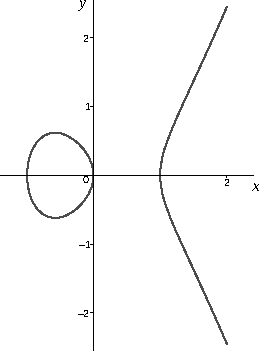
\includegraphics[width=.45\linewidth]{gfx/grafo_curva_eliptica_reales_1.pdf}} \quad
		\subfloat[$E_2: y^2 = x^3 + x$]
		{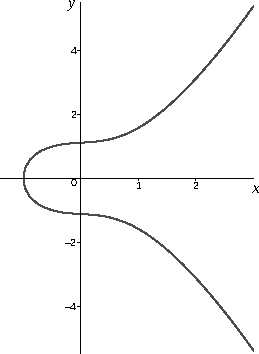
\includegraphics[width=.45\linewidth]{gfx/grafo_curva_eliptica_reales_2.pdf}}
		\caption{Curvas elípticas sobre $\mathbb{R}$}\label{fig:curvas elípticas reales}
	\end{figure}

	% \begin{figure}[h]
	% 	\centering
	% 	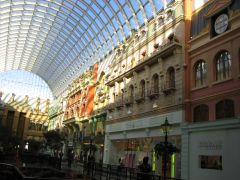
\includegraphics[scale=1]{gfx/example_1}
	% 	\caption{Curvas elípticas sobre $\mathbb{R}$}\label{fig:curvas elípticas reales}
	% \end{figure}
\end{ejemplo}

\subsection{Ecuaciones de Weierstrass simplificadas}
\label{sub:Ecuaciones de Weierstrass simplificadas}

\begin{definicion}
	Dos curvas elípticas $E_1$ y $E_2$ definidas sobre $K$ y dadas por las ecuaciones de Weierstrass:
	\begin{align*}
		E_1 &: y^2 + a_1 x y + a_3 y = x^3 + a_2 x^2 + a_4 x + a_6 \\
		E_2 &: y^2 + a_1' x y + a_3' y = x^3 + a_2' x^2 + a_4' x + a_6'
	\end{align*}
	se dicen que son \emph{isomorfas sobre K} si existen $u, r, s, t \in K,\ u \neq 0$, tal que el cambio de variables lineal
	\begin{equation}\label{eq:cambio de variables admisible}
	(x, y) \mapsto (u^2 x + r, u^3 y + u^2 s x + t)
	\end{equation}
	transforma la ecuación $E_1$ en la ecuación $E_2$. La transformación~\eqref{eq:cambio de variables admisible} se llama un cambio de variables admisible.

	El cambio de variables~\eqref{eq:cambio de variables admisible} es el único que deja <<fijo>> el punto del infinito y preserva la forma de la ecuación de Weierstrass. No vamos a entrar en más detalle, pero puede consultar~\cite[prop. III.3.1b]{Silverman:2009} para más informácion.
\end{definicion}

% TODO: explicar porqué este cambio de variable referenciando a silverman

Una ecuación de Weierstrass
$$
E:  y^2 + a_1 x y + a_3 y = x^3 + a_2 x^2 + a_4 x + a_6
$$
puede simplificarse considerablemente aplicando cambios de variables admisibles. Usaremos las ecuaciones simplificadas en vez de la general en el resto del trabajo. Vamos a considerar por separado los casos en los que el cuerpo base tenga característica distinta de 2 y 3 o tenga característica 2.

\begin{enumerate}
	\item Si la característica de $K$ es distinta de $2$ y $3$, entonces el cambio de variables admisible
	$$
	(x, y) \mapsto \left(\frac{x - 3 a_1^2 - 12 a_2}{36}, \frac{y - 3 a_1 x}{216} - \frac{a_1^3 + 4 a_1 a_2 - 12 a_3}{240}\right)
	$$
	transforma $E$ en la curva
	\begin{equation*}\label{eq:ecuación Weierstrass}
		y^2 = x^3 + a x + b
	\end{equation*}
	donde $a, b \in K$. El discriminante de esta curva es $\Delta = -16(4a^3 + 27b^2)$.

	\item Si la característica de K es 2, hay dos casos que considerar. Si $a_1 \neq 0$, entonces el cambio de variables admisible
	$$
	(x, y) \mapsto \left(a_1^2 x + \frac{a_3}{a_1}, a_1^3 y + \frac{a_1^2 a_4 + a_3^2}{a_1^3} \right)
	$$
	transforma $E$ en la curva
	\begin{equation*}
		y^2 + xy = x^3 + a x^2 + b
	\end{equation*}
	% TODO: rellenar referencia
	donde $a, b \in K$. Tales curvas se llaman \emph{no supersingulares} (véase~\ref{}) y tienen discriminante $\Delta = b$. Si $a_1 = 0$, entonces el cambio de variables admisible
	$$
	(x, y) \mapsto (x + a_2, y)
	$$
	transforma $E$ en la curva
	\begin{equation*}
		y^2 + c y = x^3 + a x + b
	\end{equation*}
	% TODO: rellenar referencia
	donde $a, b, c \in K$. Tales curvas se llaman \emph{supersingulares} (véase~\ref{}) y tienen discriminante $\Delta = c^4$.

	% \item Si la característica de $K$ es 3, entonces hay dos casos que considerar. Si $a_1^2 \neq -a_2$, entonces el cambio de variables admisible
	% $$
	% (x, y) \mapsto \left(x + \frac{d_4}{d_2}, y + a_1 x + a_1 \frac{d_4}{d_2} + a_3 \right)
	% $$
	% donde $d_2 = a_1^2 + a_2$ y $d_4 = a_4 - a_1 a_3$, transforma $E$ en la curva
	% \begin{equation*}
	% 	y^2 = x^3 + a x^2 + b
	% \end{equation*}
	% % TODO: rellenar referencia
	% donde $a, b \in K$. Tales curvas se llaman \emph{no supersingulares} (véase~\ref{}) y tiene discriminante $\Delta = -a^3 b$. Si $a_1^2 = -a_2$, entonces el cambio de variables admisible
	% $$
	% (x, y) \mapsto (x, y + a_1 x + a_3)
	% $$
	% transforma $E$ en la curva
	% \begin{equation*}
	% 	y^2 = x^3 + a x^2 + b
	% \end{equation*}
	% % TODO: rellenar referencia
	% donde $a, b \in K$. Tales curvas se llaman \emph{supersingulares} (véase~\ref{}) y tiene discriminante $\Delta = -a^3$.
\end{enumerate}
\begin{proof}
La demostración completa puede encontrarse en~\cite[sec. III.1]{Silverman:2009}. Se trata simplemente de completar cuadrados y realizar sustituciones, por ello aquí solo mostraremos la demostración de la primera simplificación.

En primer lugar, sumando en la ecuación de Weierstrass~\eqref{eq:Weierstrass general} en ambos lados por $(a_1 a_3 x)/2 + a_3^2/4 + (a_1^2 x^2)/4$, completamos el cuadrado:
$$
\left(y + \frac{a_1 x}{2} + \frac{a_3}{2}\right)^2 = x^3 + \left(a_2 + \frac{a_1^2}{4}\right)x^2 + \left(a_4 + \frac{a_1 a_3}{2}\right)x + \left(a_6 + \frac{a_3^2}{4}\right)
$$
Haciendo $y_1 = y + (a_1 x)/2 + a_3/2$, obtenemos
$$
y_1^2 = x^3 + a_2' x^2 + a_4' x + a_6'
$$
para algunas constantes $a_2', a_4', a_6' \in K$. Finalmente, sustituyendo $x_1 = x + a_2'/3$ resulta
$$
y_1^2 = x_1^3 + a x_1 + b
$$
para algunas constante $a, b \in K$. Para obtener el discriminante $\Delta$ basta sustiuir el valor de las constantes $a_4 = a,\ a_6 = b$ y $a_1 = a_3 = a_2 = 0$ en~\eqref{eq:discriminante}.
\end{proof}

\subsection{Ley de grupo}
\label{sub:Ley de grupo}

Sea $E$ una curva elíptica definida sobre un cuerpo $K$. Hay un \emph{método de la cuerda y la tangente} para sumar dos puntos en $E(K)$ y obtener un tercer punto en $E(K)$. Junto con esta operación aditiva, el conjunto de puntos $E(K)$ forma un gurpo abeliano con $\infty$ como elemento neutro.

La regla aditiva se explica fácilmente geométricamente. Sea $P$ y $Q$ dos puntos distintos de una curva elíptica $E$. Entonces la \emph{suma} $R$, de $P$ y $Q$ esta definido como sigue. Se dibuja una recta $L$ de $P$ a $Q$. Esta recta intersecta la curva elíptica en un tercer punto. Entonces $R$ es la reflexión de este punto sobre el eje-$x$. Esto se puede apreciar en la Figura~\ref{fig:ejemplo adicción}.

El \emph{doble} $R$, de $P$, se define como sigue. Se dibuja la línea tangente $L$ a la curva elíptica en $P$. Esta línea intersecta la curva elíptica en un segundo punto. Entonces $R$ es la reflexión de esto punto sobre el eje-$x$. Esto se puede apreciar en la Figura~\ref{fig:ejemplo duplicación}.

\begin{figure}[h]
  \myfloatalign
  \subfloat[Adicción: $P + Q = R$]{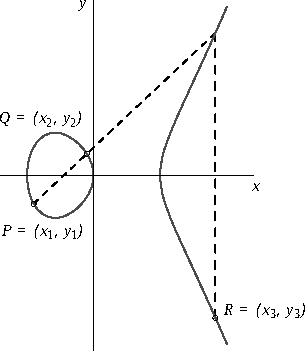
\includegraphics[width=.45\linewidth]{gfx/ejemplo_adiccion.pdf}\label{fig:ejemplo adicción}}
  \quad
  \subfloat[Duplicación: $P + P = P$]{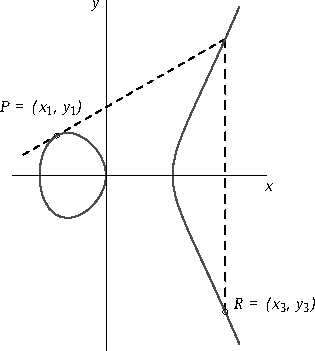
\includegraphics[width=.45\linewidth]{gfx/ejemplo_duplicacion.pdf}\label{fig:ejemplo duplicación}}
  \caption{Adicción y duplicación geométrica de puntos de una curva elíptica}\label{fig:Adicción y duplicación geométrica de puntos de una curva elíptica}
\end{figure}

El hecho de que $L \cap E$, contando multiplicidades, consiste en exactamente tres puntos (no necesariamente distintos) es un caso especial del teorema de Bézout~\cite[sec. I.7.8]{Hartshorne:1977}. Sin embargo, como vamos a dar fórmulas explícitas, no hay necesidad de usar un teorema general.

\begin{definicion}[ley de grupo]
\label{def:ley de grupo}
Sea $E$ una curva elíptica definida por la ecuación $y^2 = x^3 + a x + b$ sobre un cuerpo $K$ de característica distinta de 2 y 3. Definimos la operación binaria $+: E(K) \times E(K) \to E(K)$ como sigue:
\begin{enumerate}[label=\alph*)]
	\item $P + \infty = \infty + P = P,$ para todo $P \in E(K)$
	\item Si $P = (x, y) \in E(K)$, entonces $(x, y) + (x, -y) = \infty$. El punto $(x, -y)$ se denotará por $-P$ y se llamará el \emph{opuesto} de P. Además, $- \infty = \infty$.
	\item Sea $P = (x_1, y_1) \in E(K)$ y $Q = (x_2, y_2) \in E(K)$, donde $P \neq \pm Q$. Entonces $P + Q = (x_3, y_3)$, donde
	$$
	x_3 = \left(\frac{y_2 - y_1}{x_2 - x_1}\right)^2 - x_1 - x_2, \quad
	y_3 = \left(\frac{y_2 - y_1}{x_2 - x_1}\right) (x_1 - x_3) - y_1
	$$
	\item Sea $P = (x_1, y_1) \in E(K)$, donde $P \neq  -P$. Entonces $2 P = (x_3, y_3)$ donde:
	$$
	x_3 = \left(\frac{3 x_1^2 + a}{2 y_1}\right)^2 - 2 x_1, \quad
	y_3 = \left(\frac{3 x_1^2 + a}{2 y_1}\right) (x_1 - x_3) - y_1
	$$
\end{enumerate}
\end{definicion}
\begin{proof}
Tenemos que comprobar que $+$ es una operación binaria válida, esto es, que a cada par de elementos de $E(K) \times E(K)$ le corresponde un único elemento de $E(K)$. Como la casuística anterior es total y exclusiva, basta ver que $+$ es una operación cerrada. Los casos $a)$ y $b)$ son triviales. Veamos los otros dos casos con detalle.

\paragraph{Caso $c)$}
Supongamos $P = (x_1, y_1),\ Q = (x_2, y_2),\ P, Q \in E(K)$ con $P \neq \pm Q$. Consideramos la recta que los contiene:
$$
	L: y = m(x - x_1) + y_1,\ \text{donde}\ m = \frac{y_2 - y_1}{x_2 - x_1}
$$
Nótese que $x_2 \neq x_1$ ya que $P \neq \pm Q$. Para hallar la intersección de L con E sustituimos $y$:
$$
	(m(x - x_1) + y_1)^2 = x^3 + a x + b
$$
Podemos reescribir esto de la forma
\begin{equation}
\label{eq:cúbica}
	0 = x^3 - m^2 x^2 + b' x + c'
\end{equation}
para algunas constantes $b', c' \in K$. Así, las raíces de esta cúbica es justamente $L \cup E$.

Sabemos que las raíces de un polinomio están relacionadas con sus coeficientes. De hecho, para un polinomio cúbico mónico $x^3 + c_2 x^2 + c_1 x + c_0$ con raíces $r, s, t$ se tiene:
% -r s t  +  r s x  +  r t x  -  r x^2  +  s t x  -  s x^2  -  t x^2+x^3
\begin{align*}
	x^3 + &c_2 x^2 + c_1 x + c_0 = (x-r)(x-s)(x-t) \\
	&= x^3 - (r + s + t)x^2 + (r s + r t + s t)x - r s t
\end{align*}

En particular, $r + s + t = -c_2$. Como $P$ y $Q$ están en la intersección, $x_1$ y $x_2$ son dos raíces de~\eqref{eq:cúbica}, luego la tercera raíz $\alpha$ es $m^2 - x_1 - x_2$. Sustituyendo $\alpha$ en $L$ resulta $\beta = m(x_3 - x_1) + y_1$, luego $(\alpha, \beta) \in E(K)$. Entonces  $(\alpha, -\beta) = (x_3, y_3) \in E(K)$.

\paragraph{Caso $d)$}
Sea $P = (x_1, y_1)$, donde $P \neq -P$. Consideramos la recta tangente a $E$ en $P$
$$
	L: y = m(x - x_1) + y_1,\ \text{donde}\ m = \frac{3 x_1^2 + a}{2 y_1}
$$
Nótese que $y_1 \neq 0$ ya que si no estaríamos en el caso $b)$. Hallamos la intersección con E de forma análoga al caso $c)$ y obtenemos la cúbica:
$$
	0 = x^3 - m^2 x^2 + b' x + c'
$$
para algunas constantes $b', c' \in K$. Análogamente al caso $c)$, como $x_1$ es una raíz doble de la cúbica (derívese y evalúe en $x_1$) tenemos que la tercera raíz $\alpha$ es $m^2 - 2 x_1$. Sustituyendo $\alpha$ en $L$ resulta $\beta = m(x_3 - x_1) + y_1$, luego $(\alpha, \beta) \in E(K)$. Entonces  $(\alpha, -\beta) = (x_3, y_3) \in E(K)$.
\end{proof}

\begin{teorema}\label{th:grupo abeliano}
	La suma~\ref{def:ley de grupo} de puntos en una curva elíptica $E$ sobre un cuerpo $K$ de característica distinta de 2 y 3 satisface la siguientes propiedades:
	\begin{itemize}
		\item \emph{Conmutatividad.} $P_1 + P_2 = P_2 + P_1,\ \forall P_1, P_2 \in E(K)$.
		\item \emph{Existencia de elemento neutro.} $P + \infty = P,\ \forall P \in E(K)$.
		\item \emph{Existencia de elemento opuesto.} $P + (-P) = \infty,\ \forall P \in E(K)$.
		\item \emph{Asociatividad.} $(P_1 + P_2) + P_3 = P_1 + (P_2 + P_3),\ \forall P_1, P_2, P_3 \in E(K)$.
	\end{itemize}
	En otras palabras, $(E(K), +, \infty)$ es un grupo abeliano.
\end{teorema}
\begin{proof}
La conmutatividad es trivial en los casos $a)$, $b)$ y $d)$. Para el caso $c)$ también es fácil ya que la recta que une $P_1$ y $P_2$ es la misma que la recta que une $P_2$ y $P_1$. La existencia de elemento neutro e inverso también es directo de la definición~\ref{def:ley de grupo}.

La asociatividad puede probarse utilizando las fórmulas caso por caso, pero supone un esfuerzo demasiado laborioso. En su lugar, puede abordarse de forma más sofisticada bien estudiando las líneas y sus intersecciones con la curva elíptica en el plano proyectivo~\cite[sec. 2.4]{Washington:2008} o bien usando teoremas más generales como el de Riemann-Roch~\cite[teo. III.3.4.e]{Silverman:2009}.
\end{proof}

Hemos descrito fórmulas de adicción para curvas elípticas definidas sobre un cuerpo de característica distinta de 2 y 3. Para cuerpos con característica 2 o 3, las fórmulas cambian. Una de las principales diferencias es el opuesto de un punto. Si $E$ es una curva elíptica definida sobre un cuerpo $K$ por la ecuación general de Weierstrass~\eqref{eq:Weierstrass general}, el opuesto de un punto $P = (x, y) \in E(K)$ viene dado por
$$
	- P = (x, -a_1 x - a_3 - y)
$$
Se puede probar un teorema general al teorema~\ref{th:grupo abeliano} para curvas elípticas definidas por la ecuación general de Weierstrass~\eqref{eq:Weierstrass general} sobre cuerpos cualquier característca~\cite{Silverman:2009}. Nosotros daremos fórmulas explíticas para cuerpos finitos de característica 2 posteriormente.

% TODO: poner en el apartado cuerpos finitos
% TODO: poner tambien las supersingulares
% \begin{definicion}[ley de grupo 2]
% \label{def:ley de grupo 2}
% Sea $E$ una curva elíptica definida por la ecuación $y^2 + x y = x^3 + a x^2 + b$ sobre el cuerpo finito $\Fm$. Definimos la operación binaria $+: E(\Fm) \times E(\Fm) \to E(\Fm)$ como sigue:
% \begin{enumerate}[label=\alph*)]
% 	\item $P + \infty = \infty + P = P,$ para todo $P \in E(\Fm)$
% 	\item Si $P = (x, y) \in E(\Fm)$, entonces $(x, y) + (x, x + y) = \infty$. El punto $(x, x + y)$ se denotará por $-P$ y se llamará el \emph{opuesto} de P. Además, $- \infty = \infty$.
% 	\item Sea $P = (x_1, y_1) \in E(\Fm)$ y $Q = (x_2, y_2) \in E(\Fm)$, donde $P \neq \pm Q$. Entonces $P + Q = (x_3, y_3)$, donde
% 	$$
% 	x_3 = \lambda^2 \lambda + x_1 + x_2 + a, \quad
% 	y_3 = \lambda (x_1 + x_3) + x_3 + y_1
% 	$$
% 	con $\lambda = (y_1 + y_2)/(x_1 + x_2)$.
% 	\item Sea $P = (x_1, y_1) \in E(\Fm)$, donde $P \neq -P$. Entonces $2 P = (x_3, y_3)$ donde:
% 	$$
% 	x_3 = \lambda^2 \lambda + a = x_1^2 + b/x_1^2, \quad
% 	y_3 = x_1^2 + \lambda x_3 + x_3
% 	$$
% 	con $\lambda = x_1 + y_1/x_1$.
% \end{enumerate}
% \end{definicion}
%
% \begin{teorema}
% 	La suma~\ref{def:ley de grupo 2} de puntos en una curva elíptica $E$ sobre el cuerpo $\F2m$ satisface la siguientes propiedades:
% 	\begin{itemize}
% 		\item \emph{Conmutatividad.} $P_1 + P_2 = P_2 + P_1,\ \forall P_1, P_2 \in E(F2m)$.
% 		\item \emph{Existencia de elemento neutro.} $P + \infty = P,\ \forall P \in E(F2m)$.
% 		\item \emph{Existencia de elemento opuesto.} $P + (-P) = \infty,\ \forall P \in E(F2m)$.
% 		\item \emph{Asociatividad.} $(P_1 + P_2) + P_3 = P_1 + (P_2 + P_3),\ \forall P_1, P_2, P_3 \in E(F2m)$.
% 	\end{itemize}
% 	En otras palabras, $(E(F2m), +, \infty)$ es un grupo abeliano.
% \end{teorema}


\subsubsection{Multiplicación escalar}
\label{subs:Multiplicación escalar}

Si $P$ es un punto de una curva elíptica y $k$ un entero positivo, entonces $k P$ denotará la suma con $k$-sumandos $P + \ldots + P$. Para calcular $k P$ para un entero grande $k$, es ineficiente sumar $P$ consigo mismo repetidamente.  Es mucho más rápido usar el siguiente algoritmo:

\begin{algoritmo}[multiplicación por duplicación]
	Sea $k$ un entero positivo y sea $P$ un punto de una curva elíptica. El siguiente algoritmo calcula $kP$.
	\begin{enumerate}
		\item Se empieza con $a = k$, $B = \infty$, $C = P$.
		\item Si $a$ es par, se toma $a = a/2$ y se toma $B = B$, $C = 2 C$.
		\item Si $a$ es impar, se toma $a = a -1$, y se toma $B = B + C$, $C = C$.
		\item Si $a \neq 0$, se va al paso 2.
		\item Se devuelve $B$.
	\end{enumerate}
	La salida $B$ es $kP$.
\end{algoritmo}

El único problema de este método es que el tamaño de las coordenadas del punto pueden incrementar muy rápidamente (por ejemplo si trabajamos sobre los números racionales). Sin embargo, cuando trabajamos con un cuerpo finito, por ejemplo $\Fp$, esto no es un problema ya que podemos reducir módulo $p$ continuamente y mantener los números involucrados relativamente pequeños. Nótese que la asociatividad de la suma de puntos de una curva elíptica nos permite hacer estos cálculos sin preocuparnos del orden que usamos para combinar los sumandos.

\subsection{Forma proyectiva}
\label{sub:Forma proyectiva}

Sea $K$ un cuerpo. El \emph{espacio proyectivo} dos dimensional sobre $K$, $\P^2(K)$, esta dado por clases de equivalencia de ternas $(x, y, z)$ con $x, y, z \in K$ y al menos algún $x, y, z$ no nulo. Dos ternas $(x_1, y_1, z_1)$ y $(x_2, y_2, z_2)$ se dicen que son \emph{equivalentes} si existe un elemento no nulo $\lambda \in K$ tal que
$$
	(x_1, y_1, z_1) = (\lambda x_2, \lambda y_2, \lambda z_3)
$$
y en tal caso escribiremos $(x_1, y_1, z_1) \sim (x_2, y_2, z_2)$. La clase de equivalencia de una terna solo depende de los ratios entre $x, y, z$. Por ello, la clase de equivalencia de $(x, y, z)$ la denotaremos por $(x : y : z)$ y diremos que es un \emph{punto proyectivo}.

Si $(x : y : z)$ es un punto proyectivo con $z \neq 0$, entonces $(x : y : z) = (x/z : y/z : 1)$ y de hecho $(x/z, y/z, 1)$ es el único representante de esta clase de equivalencia con $z = 1$. Tenemos así una correspondencia $1-1$ entre el conjunto de puntos proyectivos
$$
	\P^2(K)^* = \left\{(x : y : z) : x, y, z \in K,\ z \neq 0 \right\}
$$
y el \emph{plano afín}
$$
	\A(K) = \left\{(x, y) : x, y \in K \right\}.
$$

Si $z = 0$, el conjunto de puntos proyectivos de la forma $(x : y : 0)$ se llaman \emph{recta del infinito} ya que sus puntos no se corresponden con ningúno del plano afín.

La \emph{forma proyectiva} de una ecuación de Weierstrass de una curva elíptica $E$ definida sobre $K$ se obtiene remplazando $x$ por $x/z$, $y$ por $y/z$ y quitando denominadores. Si alguna terna $(x, y, z)$ no nula satisface la ecuación proyectiva entonces también las satisfacen las ternas $(x', y', z') \in (x : y : z)$. Podemos decir entonces que un punto proyectivo $(x : y : z)$ está en $E$. Tenemos así una correspondencia 1-1 entre los puntos del plano afín que están en $E$ y los puntos proyectivos de $P^2(K)^*$ que están en $E$.

Si hacemos $z = 0$ en la forma proyectiva de la ecuación, obtenemos $0 = x^3$ y como alguna componente tiene que ser no nula, tenemos $y \neq 0$. Así, el único punto de la recta del infinito que está en $E$ es el punto $(0 : y : 0) = (0 : 1 : 0)$. Este pusto se corresponde con el punto $\infty$ de la definición~\ref{def:curva elíptica}.

Hay situaciones en la que usar coordenadas proyectivas puede ser ventajoso (véase~\cite[sec 2.6]{Washington:2008}). Sin embargo, nosotros utilizaremos las coordenadas del plano afín, tratando el punto del infinito como un caso especial cuando sea necesario.

%**************************
\chapter{Desarrollo informático}
\label{ch:Desarrollo informático}
%**************************

% TODO: completar introducción
En este capítulo haremos el desarrollo informático sobre criptografía con curvas elípticas. En el apartado~\ref{} hablaremos sobre protocolos criptográficos y explicaremos la implementación del programa desarrollado en el apartado~\ref{}.

% TODO: añadir ref si se utilizán más
Las referencias utilizadas para el desarrollo informático han sido sido~\cite{Hankerson:2003} y~\cite{Washington:2008}.

% TODO: ver si hacer una introducción de criptografía.

\section{Protocolos criptográficos}
\label{sec:Protocolos criptográficos}

% TODO: intro

\subsection{Problema del logaritmo discreto}
\label{sub:Problema del logaritmo discreto}

La dificultad del problema del logaritmo discreto es esencial para la seguridad de los esquemas criptográficos sobre curvas elípticas.

\begin{definicion}
    El \emph{problema del logaritmo discreto sobre curvas elípticas (ECDLP)} es: dado una curva elíptica $E$ definida sobre un cuerpo finito $\Fq$, un punto $P \in E(\Fq)$ de orden $n$ y un punto $Q \in <P>$, encontrar el entero $k \in [0, n - 1]$ tal que $Q = k P$. El entero $k$ se llama el \emph{logaritmo discreto de $Q$ respecto a la base $P$} y se denota $k = \log_p Q$.
\end{definicion}

Los parámetros de una curva elíptica para los esquema criptográficos deben ser elegidos con cuidado para resistir todos los ataques conocidos sobre el ECDLP.

El ataque más simple es el ataque por \emph{fuerza bruta}: probar todos los valores posibles de $k$ hasta dar con el válido. El tiempo de ejecucción es aproximadamente $n$ pasos en el peor caso y $n / 2$ pasos en el caso medio. Así, el ataque por fuerza bruta puede ser evitado tomando curvas elípticas con $n$ suficientemente largo (p. ej. $n > 2^{80}$).

El mejor ataque de propósito general conocido sobre el ECDLP es la combinación del \emph{algoritmo de Pohlig-Hellman} y del \emph{algoritmo rho de Pollard}, que tiene un complejidad temporal exponencial de $O(\sqrt{p})$ donde $p$ es el divisor primo más grande de $n$. Para resistir este ataque, se debe elegir curvas elípticas tal que $n$ sea divisible por un primo $p$ suficiente grande (p. ej $p > 2^{160}$).

Además se deben evitar ciertos tipos de curvas para los cuales existen ataques específicos más rápidos que el algoritmo rho de Pollard. Así pues, se deben evitar las curvas \emph{anómalas} (cuyo orden es de la forma $|E(\Fp)| = p$), curvas supersingulares (véase ~\ref{def:supersingular}), curvas con un orden de la forma $|E(\Fq)| = q - 1$ y curvas sobre $\Fm$ si $m$ es compuesto.

Puede encontrar una descripción de estos ataques en~\cite[cap. 4]{Hankerson:2003} y en~\cite[cap. 4]{Washington:2008}.

%**************************
\chapter{Conclusiones y vías futuras}
\label{ch:Conclusiones y vías futuras}
%**************************

% Las conclusiones deberán incluir todas aquellas de tipo profesional y académico. Además, se deberá indicar si los objetivos han sido alcanzados totalmente, parcialmente o no alcanzados.
%
% Si hubiese posibles vías claras de desarrollo posterior sería interesante destacarlas aquí, poniéndolas en valor en el contexto inicial del trabajo.
%
% Finalmente vienen las conclusiones y recomendaciones, en las que, a partir de lo planteado en las secciones anteriores, se presentan los resultados del trabajo, según las hipótesis de partida que se exponían en la introducción. Según los casos, aquí se pueden incluir recomendaciones prácticas y futuras líneas de investigación.

Como hemos visto, la teoría de curvas elípticas es una teoría rica, sofisticada y extensa. Sin embargo, uno de sus aspectos más sorprendentes es su aplicación en la criptografía y como supone una mejora de los sistemas criptográficos ampliamente utilizados. Esta aplicación es un muy buen ejemplo de campo interdisciplinar entre las matemáticas y las ciencias de la computación.

Los objetivos propuestos inicialmente se han alcanzando en su totalidad, sin embargo, la criptografía con curvas elípticas abarca mucho más de lo tratado en este trabajo. Existen así numerosas vías de desarrollo posterior, en la que destacamos algunas:
\begin{itemize}
    \item La \emph{criptografía basada en identidad}, cuyos esquemas criptográficos más utilizados se basan en los emparejamientos bilineales de curvas elípticas, como el emparejamiento Weil estudiado en la sección~\ref{subs:Emparejamiento Weil}.
    \item Un estudio más profundo acerca de los ataques sobre el problema del logaritmo discreto con curvas elípticas estudiado en el apartado~\ref{sub:Problema del logaritmo discreto}. Como ya explicamos, la seguridad de los sistemas criptográficos viene determinada por los ataques conocidos y en este trabajo se realizó una mera introducción sobre ellos. Estos ataques presenten ideas muy interesantes y usan resultados sutiles para conseguir la mayor eficiencia.
    \item Las curvas hiperelípticas, una generalización de las curvas elípticas, y su aplicación en la criptografía. Como ya comentamos en la introducción, aún no se han conseguido sistemas basados en curvas hiperelípticas bien más seguros o bien más eficientes que los basados en curvas elípticas. Aún así, es un campo muy reciente y con gran camino por recorrer.
    \item Desarrollo de algoritmos más eficientes. Mucha de la investigación actual sobre criptografía con curvas elípticas se basa en la búsqueda de algoritmos más eficientes para mejorar la velocidad de estos sistemas. Así, se podría hacer un estudio del estado del arte y desarrollar un nuevo algoritmo que suponga un avance en este ámbito.
\end{itemize}

%\include{multiToC} % <--- just debug stuff, ignore for your documents
% ********************************************************************
% Backmatter
%*******************************************************
\appendix
%\renewcommand{\thechapter}{\alph{chapter}}
\cleardoublepage
%********************************************************************
% Apéndice
%*******************************************************
\chapter{Apéndice}
\label{ap:apendice}

% If problems with the headers: get headings in appendix etc. right
%\markboth{\spacedlowsmallcaps{Appendix}}{\spacedlowsmallcaps{Appendix}}

\begin{center}
  \spacedlowsmallcaps{Estudio del cifrado de algunas páginas web de la Universidad de Granada}
\end{center}

Como aplicación del estudio teórico-práctico realizado en los capítulos \ref{ch:Desarrollo matemático} y \ref{ch:Desarrollo informático}, hemos considerado de interés hacer un estudio preliminar sobre el cifrado de algunas páginas web de la Universidad de Granada.

En un primer momento pensábamos que, en atención a las políticas de seguridad y no difusión de datos personales, aquellas páginas que tienen acceso a información reservada estaban protegidas. Sin embargo, hemos comprobado que algunas de ellas presentan vulnerabilidades.

Un listado de las páginas visitadas a fecha 30/03/2016 junto con los fallos de seguridad encontrados se presenta a continuación.

\section*{Páginas web vulnerables}

\subsection*{Primer fallo de seguridad encontrado}

El primer y principal fallo de seguridad que hemos encontrado ha sido la inexistencia de cifrado en el envío de credenciales de las siguientes páginas web:

\begin{itemize}
  \setlength\itemsep{0.1em}
  \item \url{http://fciencias.ugr.es}
  \item \url{http://etsiit.ugr.es}
  \item \url{http://grados.ugr.es/informaticaymatematicas}
  \item \url{http://grados.ugr.es/informatica}
  \item \url{http://grados.ugr.es/matematicas}
  \item \url{http://sucre.ugr.es} (incluyendo \url{http://fciencias.ugr.es/aulas/} y la página de reserva de aulas accesible via \url{http://etsiit.ugr.es})
  \item \url{http://calidad.ugr.es}
  \item \url{http://secretariageneral.ugr.es}
  \item \url{http://archivo.ugr.es}
  \item \url{http://catedras.ugr.es}
  \item \url{http://cicode.ugr.es}
  \item \url{http://editorial.ugr.es}
  \item \url{http://unidadigualdad.ugr.es}
  \item \url{http://biotic.ugr.es/pages/intranet}
  \item \url{http://internacional.ugr.es}
  \item \url{http://ssprl.ugr.es}
\end{itemize}

Las páginas anteriores disponen de un apartado de \emph{login} y como solo está disponible el protocolo \code{HTTP}  en vez del protocolo \code{HTTPS} , las credenciales podrían ser interceptadas por un usuario malicioso.

Como caso real, supongamos un usuario conectado a la \emph{cvi-ugr} o a otra red wifi pública. Si este ingresara sus credenciales en alguna de las páginas anteriores y en ese momento hubiera un usuario malicioso analizando los paquetes de la red, el usuario malicioso obtendría fácilmente sus credenciales. De hecho, hoy en día existen programas como Wireshark que hacen del análisis de paquetes una tarea muy sencilla.

La solución a este fallo de seguridad es deshabilitar \code{HTTP}  y utilizar para estas páginas \code{HTTPS}  exclusivamente.

Además, suponemos que la lista es mucho más extensa, ya que:
\begin{itemize}
  \item Al igual que \href{http://fciencias.ugr.es}{fciencias.ugr.es} y \href{http://etsiit.ugr.es}{etsiit.ugr.es}, las páginas web de muchos otros centros presentan el mismo fallo.
  \item Al igual que \href{http://grados.ugr.es/informatica}{grados.ugr.es/informatica}, \href{http://grados.ugr.es/matematicas}{grados.ugr.es/matematicas} y \href{http://grados.ugr.es/informaticaymatematicas}{grados.ugr.es/informaticaymatematicas}, las páginas web de muchos otros grados presentan el mismo fallo.
\end{itemize}

\subsection*{Segundo fallo de seguridad encontrado}

El segundo fallo de seguridad que hemos encontrado ha sido la coexistencia de envío de credenciales cifradas y no cifradas de las siguientes páginas web:

\begin{itemize}
  \setlength\itemsep{0.1em}
  \item \url{http://oficinavirtual.ugr.es/ai}
  \item \url{http://sede.ugr.es/sede/mis-procedimientos/index.html} (eligiendo sin certificado digital)
\end{itemize}
Las páginas anteriores se pueden usar tanto con el protocolo \code{HTTP}  como con el protocolo \code{HTTPS} . De este modo, si se utilizan con el protocolo \code{HTTP}  presentan el mismo fallo que el anterior conjunto de páginas web.

La solución es más sencilla ya que al estar implementado el acceso por \code{HTTPS}  para estas web, solo hay que deshabilitar \code{HTTP}, dejando  \code{HTTPS}  como la única opción.

Nótese que aunque este listado es más breve contiene una de las páginas más críticas de la UGR, \href{http://oficinavirtual.ugr.es/ai}{oficinavirtual.ugr.es/ai}.

%********************************************************************
% Other Stuff in the Back
%*******************************************************
\cleardoublepage%********************************************************************
% Bibliografía
%*******************************************************

% Se incluirán tanto las fuentes primarias como todas aquellas cuyo peso haya sido menor en la realización del trabajo. Se recomienda un breve comentario de las referencias, ya sea individualizado, por grupos de referencias o global. En caso de incluir URLs de páginas web deberán ir acompañadas de título, autor y fecha de último acceso, entre otros datos relevantes. Se recomienda no abusar de este tipo de fuentes.


% work-around to have small caps also here in the headline
\manualmark
\markboth{\spacedlowsmallcaps{\bibname}}{\spacedlowsmallcaps{\bibname}} % work-around to have small caps also
%\phantomsection
\refstepcounter{dummy}
\addtocontents{toc}{\protect\vspace{\beforebibskip}} % to have the bib a bit from the rest in the toc
\addcontentsline{toc}{chapter}{\tocEntry{\bibname}}
\label{app:bibliography}

\printbibliography

% TODO: escribir comentario de bibliografía

\section*{Referencias web}

% TODO: añadir referencias web

% ********************************************************************
% Game Over: Restore, Restart, or Quit?
%*******************************************************
\end{document}
% ********************************************************************
